%definira klasu dokumenta 
\documentclass[12pt]{report} 

%prostor izmedu naredbi \documentclass i \begin{document} se zove uvod. U njemu se nalaze naredbe koje se odnose na cijeli dokument

%osnovni LaTex ne može riješiti sve probleme, pa se koriste različiti paketi koji olakšavaju izradu željenog dokumenta
\usepackage[croatian]{babel} 
\usepackage{amssymb}
\usepackage{amsmath}
\usepackage{txfonts}
\usepackage{mathdots}
\usepackage{titlesec}
\usepackage{array}
\usepackage{lastpage}
\usepackage{etoolbox}
\usepackage{tabularray}
\usepackage{color, colortbl}
\usepackage{adjustbox}
\usepackage{geometry}
\usepackage[classicReIm]{kpfonts}
\usepackage{hyperref}
\usepackage{fancyhdr}

\usepackage{float}
\usepackage{setspace}
\restylefloat{table}


\patchcmd{\chapter}{\thispagestyle{plain}}{\thispagestyle{fancy}}{}{} %redefiniranje stila stranice u paketu fancyhdr

%oblik naslova poglavlja
\titleformat{\chapter}{\normalfont\huge\bfseries}{\thechapter.}{20pt}{\Huge}
\titlespacing{\chapter}{0pt}{0pt}{40pt}


\linespread{1.3} %razmak između redaka

\geometry{a4paper, left=1in, top=1in,}  %oblik stranice

\hypersetup{ colorlinks, citecolor=black, filecolor=black, linkcolor=black,	urlcolor=black }   %izgled poveznice


%prored smanjen između redaka u nabrajanjima i popisima
\newenvironment{packed_enum}{
	\begin{enumerate}
		\setlength{\itemsep}{0pt}
		\setlength{\parskip}{0pt}
		\setlength{\parsep}{0pt}
	}{\end{enumerate}}

\newenvironment{packed_item}{
	\begin{itemize}
		\setlength{\itemsep}{0pt}
		\setlength{\parskip}{0pt}
		\setlength{\parsep}{0pt}
	}{\end{itemize}}




%boja za privatni i udaljeni kljuc u tablicama
\definecolor{LightBlue}{rgb}{0.9,0.9,1}
\definecolor{LightGreen}{rgb}{0.9,1,0.9}

%Promjena teksta za dugačke tablice
\DefTblrTemplate{contfoot-text}{normal}{Nastavljeno na idućoj stranici}
\SetTblrTemplate{contfoot-text}{normal}
\DefTblrTemplate{conthead-text}{normal}{(Nastavljeno)}
\SetTblrTemplate{conthead-text}{normal}
\DefTblrTemplate{middlehead,lasthead}{normal}{Nastavljeno od prethodne stranice}
\SetTblrTemplate{middlehead,lasthead}{normal}

%podesavanje zaglavlja i podnožja

\pagestyle{fancy}
\lhead{Programsko inženjerstvo}
\rhead{Nestali ljubimci}
\lfoot{I'm a teapot}
\cfoot{stranica \thepage/\pageref{LastPage}}
\rfoot{\today}
\renewcommand{\headrulewidth}{0.2pt}
\renewcommand{\footrulewidth}{0.2pt}


\begin{document} 
	
	
	
	\begin{titlepage}
		\begin{center}
			\vspace*{\stretch{1.0}} %u kombinaciji s ostalim \vspace naredbama definira razmak između redaka teksta
			\LARGE Programsko inženjerstvo\\
			\large Ak. god. 2023./2024.\\
			
			\vspace*{\stretch{3.0}}
			
			\huge Nestali ljubimci\\
			\Large Dokumentacija, Rev. \textit{1}\\
			
			\vspace*{\stretch{12.0}}
			\normalsize
			Grupa: \textit{I'm a teapot}\\
			Voditelj: \textit{Nora Ivić}\\
			
			
			\vspace*{\stretch{1.0}}
			Datum predaje: \textit{$<$dan$>$. $<$mjesec$>$. $<$godina$>$.}\\
	
			\vspace*{\stretch{4.0}}
			
			Nastavnik: \textit{Alan Jović}\\
		
		\end{center}

	
	\end{titlepage}

	
	\tableofcontents


	\chapter{Dnevnik promjena dokumentacije}
				
		
		\begin{longtblr}[
				label=none
			]{
				width = \textwidth, 
				colspec={|X[2]|X[13]|X[3]|X[3]|}, 
				rowhead = 1
			}
			\hline
			\textbf{Rev.}	& \textbf{Opis promjene/dodatka} & \textbf{Autori} & \textbf{Datum}\\[3pt] \hline
			0.1 & Napravljen predložak.	& Marta Matulić & 20.10.2023. 		\\[3pt] \hline 
			0.2 &  Aktori i funkcionalni zahtjevi. &  Marta Matulić, Ivan Žinić & 26.10.2023. \\[3pt] \hline	
			0.3 & Dodan opis zadatka.\newline Ubačene slike sličnih rješenja. & Marta Matulić, Ivan Žinić & 27.10.2023. 	\\[3pt] \hline  
			0.4 & Dodani opisi obrazaca uporabe. & Marta Matulić, Ivan Žinić & 29.10.2023. \\[3pt] \hline
			0.4.1 & Dodani novi obrasci uporabe. & Ivan Žinić & 31.10.2023. \\[3pt] \hline
			0.5 & Ostali zahtjevi. \newline Ispravak opisa zadatka. & Marta Matulić, Ivan Žinić & 01.11.2023. \\[3pt] \hline
			0.6 & Dijagrami baze podataka. & Marta Matulić & 04.11.2023. \\[3pt] \hline
			0.7 & Dijagrami obrazaca uporabe. \newline Sekvencijski dijagrami. & Marta Matulić, Ivan Žinić & 05.11.2023. \\[3pt] \hline
			0.7.1 &Ispravak opisa zadatka.  & Marta Matulić & 08.11.2023. \\[3pt] \hline
			0.8 & Opis baze podataka. \newline Opis tablica baze. & Ivan Žinić & 10.11.2023. \\[3pt] \hline
			0.9 & Opis arhitekture sustava. & Marta Matulić & 10.11.2023. \\[3pt] \hline
			0.9.1 & Dopuna arhitekture sustava. & Marta Matulić & 11.11.2023. \\[3pt] \hline
			0.9.2 & Ispravak opisa i dijagrama baze. \newline Ispravak opisa zadatka. & Marta Matulić, Ivan Žinić & 15.11.2023. \\[3pt] \hline
			0.10 & Dijagrami razreda. \newline Opis dijagrama razreda. & Marta Matulić, Ivan Žinić & 17.11.2023. \\[3pt] \hline
			\textbf{1.0} & Ispravak pravopisnih grešaka. \newline Gotova prva verzija dokumentacije. & Marta Matulić, Ivan Žinić & 17.11.2023. \\[3pt] \hline
			1.1 & Korištene tehnologije i alati. & Marta Matulić & 08.01.2024. \\[3pt] \hline
			1.2 & Zaključak i budući rad. & Ivan Žinić & 09.01.2024. \\[3pt] \hline
			1.3 & Dijagram aktivnosti. & Marta Matulić & 09.01.2024. \\[3pt] \hline
			1.4 & Druga revizija dijagrama razreda. & Marta Matulić & 13.01.2024. \\[3pt] \hline
			1.5 & Dijagram stanja. \newline Dijagram razmještaja. & Ivan Žinić & 14.01.2024. \\[3pt] \hline
			1.6 & Dijagram komponenti. & Marta Matulić & 15.01.2024. \\[3pt] \hline
			1.6.1 & Dupuna dijagrama stanja. \newline Dopuna dijagrama razmještaja. & Ivan Žinić & 16.01.2024. \\[3pt] \hline
			1.6.2 & Dupuna dto dijagrama razreda. \newline Dopuna repository dijagrama razreda. & Ivan Žinić & 17.01.2024. \\[3pt] \hline
			1.7 & Testiranje komponenti. & Marta Matulić & 18.01.2024. \\[3pt] \hline
			1.7.1 & Dopuna view dijagrama razreda. & Marta Matulić & 18.01.2024. \\[3pt] \hline

		\end{longtblr}
	
	
	\chapter{Opis projektnog zadatka}
		
		Velik broj kućnih ljubimaca iz raznih razloga odluta od svojih vlasnika. Jako ih je teško samostalno pronaći, pogotovo u velikim gradovima s mnogo ljudi i gustim prometom. Kako je nepraktično oglašavati njihove nestanke, opažanja i pronalaske s preciznim podacima putem uobičajenih internetskih platformi za komunikaciju koje nisu razvijene s ovom namjenom (npr. društvene mreže, stranice za oglašavanje i sl.), potrebno je razviti jednostavnu i korisnu aplikaciju koja će vlasnicima kućnih ljubimaca, skloništima za životinje, ali i drugim uključenim ljudima olakšati rješavanje ovih stresnih situacija. Tako će napokon svi podaci o nestancima, opažanjima i pronalascima biti okupljeni na jednome mjestu, umjesto kao do sada raspršeni. Osobi će pri pronalasku ili nestanku ljubimca obavještavanje ostalih brižnih vlasnika i drugih ljudi biti udaljeno samo nekoliko klikova. Naša aplikacija razvija se upravu u tu svrhu. U današnje vrijeme kad je tehnologija lako i široko dostupna, gotovo svi imaju mobilne uređaje pri ruci u svakom trenutku. Zato će aplikacija biti ciljano razvijena za mobilne uređaje, te će za sve dionike u ovom procesu podržavati što veću brzinu reagiranja, koja je često ključna za uspješan završetak potrage za kućnim ljubimcem. Nadamo se da će aplikacija pomoći ponovo ujediniti što je moguće više vlasnika s njihovim sretno pronađenim ljubimcima, te na jednom mjestu okupiti sve ljude koji su voljni pomoći u potragama. 

Slična aplikacija čije su slike dane kao primjer je američka aplikacija „MissingPetFinder“ koja je prilagođena korisnicima na njihovom području.  Njihova aplikacija ne nudi opciju skloništa, već je prilagođena isključivo za osobnu upotrebu. Također nudi dodatne opcije poput printanja letaka i slanja notifikacija koje za sada naša aplikacija ne nudi, iako je takva nadogradnja moguća ukoliko bi se pokazalo korisnim.

Aplikacija treba podržavati rad tri tipa korisnika:

		\begin{packed_item}
			
			\item  Neregistrirani korisnik
			\item  Registrirani korisnik
			\item  Sklonište
			
		\end{packed_item}

		Prvi tip je \underbar{\textbf{neregistrirani korisnik}}. Pri ulasku u aplikaciju prikazuje mu se popis svih trenutno aktivnih oglasa o nestalim ljubimcima i osnovnim informacijama o njima (ime ljubimca, slike i broj mobitela vlasnika). Primjer sličnog rješenja nalazi se na slici ispod (slika \ref{fig:slika1}).

		%unos slike
		\begin{figure}[H]
			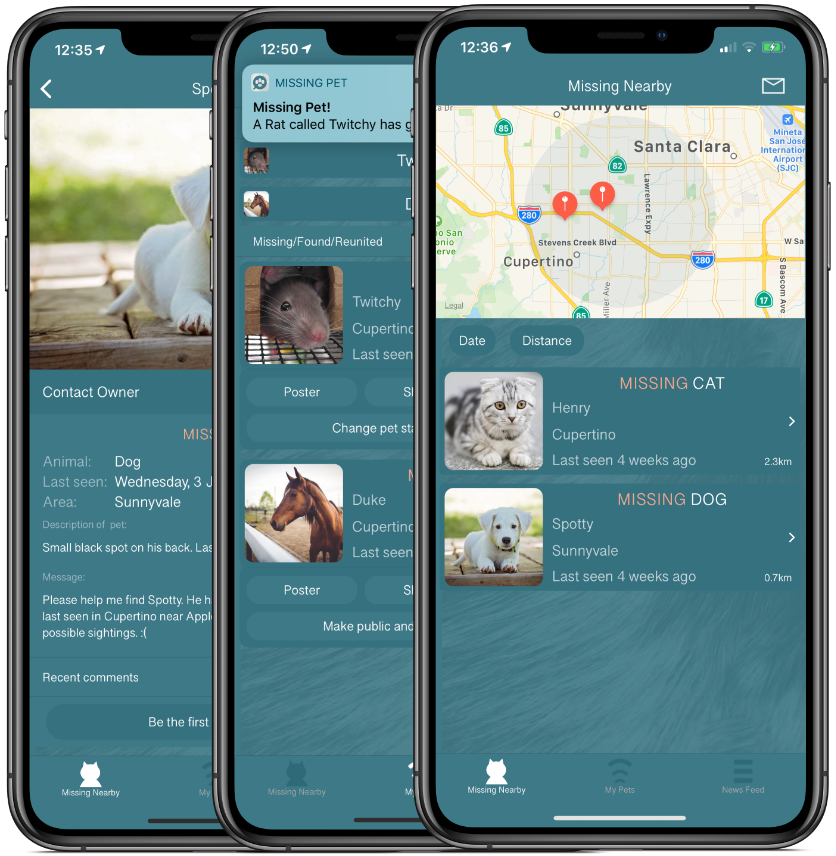
\includegraphics[scale=0.4]{slike/ljubimci.PNG} %veličina slike u odnosu na originalnu datoteku i pozicija slike
			\centering
			\caption{Primjer sličnog rješenja}
			\label{fig:slika1}
		\end{figure}

		Takav korisnik može i pretraživati oglašene nestale kućne ljubimce i skloništa za životinje. Pretraživanje je omogućeno po svim kategorijama podataka o ljubimcu koje su dostupne pri oglašavanju (vidi dolje), kao i po nazivu skloništa. Također, odabirom nekog od kućnih ljubimaca otvara se mogućnost detaljnijeg pregleda informacija o njemu (sve informacije unesene pri objavi oglasa) kao i pregled dosadašnje komunikacije oko potrage za ljubimcem.
Ako želi sudjelovati u potrazi za ljubimcem davanjem nekih informacija, neregistrirani korisnik se treba \underbar{registrirati}. Pri registraciji on unosi potrebne podatke kako bi kreirao svoj korisnički račun:

		\begin{packed_item}
			
			\item  Korisničko ime
			\item  Lozinka
			\item  Ime
			\item  Prezime
			\item  E-mail adresa
			\item  Broj mobitela
			
		\end{packed_item}

		Ako je uspješno unio sve podatke, registracija je uspješno provedena i korisnik je stvorio svoj profil u aplikaciji. U suprotnome će aplikacija zahtijevati ponovni unos podataka.

Drugi tip korisnika aplikacije je \underbar{\textbf{ registrirani korisnik}}. On je u prošlosti već stvorio svoj profil. Pri ulasku u aplikaciju on odabire opciju za prijavu te unosi svoje korisničko ime i lozinku. Uspješna prijava omogućuje mu pristup dodatnim stavkama ove aplikacije. On, kao i neregistrirani korisnik ima opciju pregleda i pretraživanja oglasa, no njemu su pri pretraživanju dodatno dostupni ne samo aktivni, nego svi postojeći oglasi bez obzira koja im je kategorija oglasa postavljena. Osim ovih funkcija, nakon prijave korisnik također može i:

		\begin{packed_enum}
			
			\item  postaviti oglas o nestalom kućnom ljubimcu 
			\item  sudjelovati u komunikaciji oko potrage za ljubimcem 
			\item  ukloniti oglas o nestalom kućnom ljubimcu 
			\item  izmijeniti oglas o nestalom kućnom ljubimcu 
			
		\end{packed_enum}

		Takvom korisniku dostupna je opcija pregleda vlastitih oglasa. Kada ju odabere može pregledati sve oglase koje je on objavio, te mu postaju dostupne opcije za uklanjanje i izmjenu oglasa.

		Kada želi prijaviti nestanak ljubimca, korisnik odabire opciju postavljanja novog oglasa. \underbar{Postavljanje oglasa} uključuje unos sljedećih kategorija podataka:

		\begin{packed_item}
			
			\item  Vrsta
			\item  Ime na koje se odaziva
			\item  Datum i sat nestanka
			\item  Lokacija nestanka (bilježi se koristeći vanjsku uslugu za geolociranje)
			\item  Boja
			\item  Starost
			\item  Tekstni opis
			\item  Slika (maksimalno tri po oglasu)
			
		\end{packed_item}

		Oglas, osim ovih podataka, sadrži i kontakt podatke korisnika koji se automatski povlače iz korisničkih podataka danih pri registraciji (za običnog korisnika to su e-pošta i broj telefona, a dodatno za skloništa povlači se i naziv skloništa). Aplikacija pri unosu automatski provjerava je li korisnik unio sve podatke ispravno. Ako je unos ispravan, oglas je objavljuje i postaje dostupan svim korisnicima, a u protivnome se korisnik obavještava o grešci i od njega se traži ponovni upis podataka.

Kao i neregistrirani korisnik, nakon prijave korisnik može odabrati bilo koji oglas i klikom na njega dobiti više informacija o tom ljubimcu (slika \ref{fig:slika2}), kao i pregled dotadašnje komunikacije o potrazi. No, za razliku od neregistriranog, sada korisnik može i sudjelovati u komunikaciji ako misli da ima bilo kakvu korisnu informaciju (slika \ref{fig:slika3}). Komunikacija omogućuje unos tekstualne poruke (npr. obavijestiti vlasnika o pronalasku ili pojavi sličnog ljubimca, zatražiti više informacija ako nije siguran i slično), slike i slanje geolokacije (putem vanjske usluge, isto kao i kod postavljanja oglasa). Pri slanju bilo koje informacije aplikacija također automatski bilježi i kontakt podatke osobe koja informaciju šalje.

		\begin{figure}[H]
			\centering
			\begin{minipage}{.5\textwidth}
	 			 \centering
				  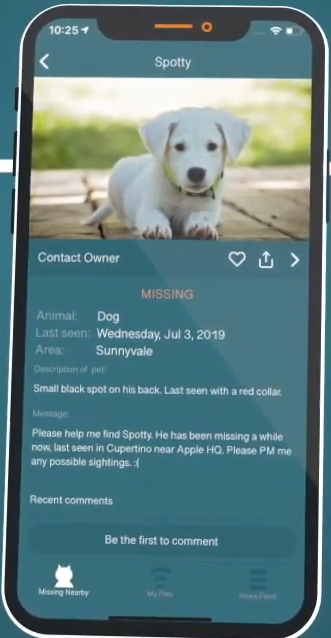
\includegraphics[width=.4\linewidth]{slike/viseInformacija.PNG}
				  \caption{Prikaz više informacija o ljubimcu kod sličnog rješenja}
				  \label{fig:slika2}
			\end{minipage}%
			\begin{minipage}{.5\textwidth}
				  \centering
				  
\includegraphics[width=.5\linewidth]{slike/Komunikacija.PNG}
				  \caption{Komunikacija kod sličnog rješenja}
				  \label{fig:slika3}
			\end{minipage}
		\end{figure}

		Iz bilo kojih razloga, korisnik uvijek ima mogućnost \underbar{ukloniti oglas} koji je sa svoga profila postavio. Uklanjanjem oglasa određeni oglas i sva njegova komunikacija nestati će iz popisa vidljivih oglasa, ali se oglas ne briše iz baze podataka. Tako on više neće biti dostupan ni njemu ni drugim korisnicima na pregled.

Registriranom korisniku nudi se i opcija izmjene oglasa koje je on postavio. \underbar{Izmjena oglasa} omogućuje izmjenu svih kategorija podataka o ljubimcu (navedeni gore kod postavljanja oglasa). Moguće je izmijeniti i kategoriju oglasa. Izbor kategorija oglasa uključuje:

		\begin{packed_enum}
			
			\item  Za ljubimcem se traga
			\item  Ljubimac je sretno pronađen
			\item  Ljubimac nije pronađen, ali je potraga obustavljena
			\item  Ljubimac je pronađen uz nesretne okolnosti
			
		\end{packed_enum}

		Po izvornim postavkama, pri objavi oglasa kategorija je automatski namještena da se za ljubimcem trenutno traga. Svaka izmjena kategorije oglasa u onu koja nije da se za ljubimcem aktivno traga automatski prebacuje oglas u popis neaktivnih oglasa, koji mogu pretraživati samo registrirani korisnici. 

Treći tip korisnika su \underbar{\textbf{skloništa za životinje}}. Skloništa za životinje su specijalni tip registriranih korisnika. Pri registraciji, kada se želi stvoriti profil za sklonište, potrebno je odabrati opciju „sklonište“. Unose se iste informacije kao i pri registraciji običnog korisnika, osim što se umjesto imena i prezimena osobe bilježi naziv skloništa. Prijava funkcionira isto kao i kod prijave običnih korisnika. U aplikaciji skloništa imaju dostupne sve opcije koje se nude i registriranim korisnicima (pregled i pretraživanje, postavljanje, uklanjanje i izmjena oglasa, te komunikacija oko potrage). Međutim, zbog toga što skloništa predstavljaju privremeni dom za mnoge tek pronađene ljubimce, kako bi se vlasnicima olakšalo lociranje njihovih ljubimaca, skloništa imaju i dodatnu mogućnost oglašavanja životinja koje su pronašli i koje se nalaze u njihovom prostoru. Zato skloništa pri postavljanju oglasa imaju ponuđenu i dodatnu opciju „u skloništu“ kojima tražene vlasnike obavještavaju da je ljubimac privremeno smješten kod njih, te čeka da vlasnici dođu po njega. Također, ako pronađu ljubimca čiji oglas već postoji, kada odaberu pregled detalja tog oglasa nudi im se opcija da označe da se taj ljubimac nalazi kod njih.

Ukoliko se aplikacija pokaže korisnom, nudi i brojne mogućnosti nadogradnje. Moguće bi bilo proširenje informacija koje se bilježe o ljubimcima, formiranje grupa za razgovor među vlasnicima koje bi mogle poslužiti i kao utjeha tijekom potrage za ljubimcima, dodavanje opcije videa, nagrada za pronalazak ljubimca ako vlasnik to želi, slanje obavijesti o nestancima u blizini i još mnogo drugih opcija.

		\eject
		
		
	\chapter{Specifikacija programske potpore}
		
	\section{Funkcionalni zahtjevi}
			
			\textbf{\textit{dio 1. revizije}}\\
			
			\noindent \textbf{Dionici:}
			
			\begin{packed_enum}
				
				\item Neregistrirani korisnik
				\item Registrirani korisnik
				\begin{packed_item}
					\item[a)] Klijent
					\item[b)] Sklonište
				\end{packed_item}
				\item Razvojni tim
				
			\end{packed_enum}
			
			\noindent \textbf{Aktori i njihovi funkcionalni zahtjevi:}
			
			
			\begin{packed_enum}
				\item  \underbar{Neregistriran/neprijavljen korisnik (inicijator) može:}
				\begin{packed_enum}
					\item pregledavati aktivne oglase
					\item pretraživati aktivne oglase
					\item registrirati se
					\item prijaviti se u sustav (za postojećeg korisnika)
					\item detaljnijije pregledati oglas i komunikacije
				\end{packed_enum}
			
				\item  \underbar{Klijent (inicijator) može:}
				\begin{packed_enum}
					\item pregledavati sve oglase
					\item pretraživati sve oglase
					\item detaljnije pregledati oglas i komunikacije
					\item komunikacirati u vezi potrage
					\item ukloniti oglas
					\item izmjeniti oglas
				\end{packed_enum}
				
				\item  \underbar{Sklonište (inicijator) može:}
				\begin{packed_enum}
					\item pregledavati sve oglase
					\item pretraživati sve oglase
					\item detaljnijije pregledati oglas i komunikacije
					\item komunicirati u vezi potrage
					\item ukloniti oglas
					\item izmijeniti oglasa
					\item postaviti oglas o ljubimcu u skloništu
				\end{packed_enum}
				
				\item  \underbar{Baza podataka (sudionik) može:}
				\begin{packed_enum}
					\item pohranjivati sve podatke o korisničkim računima
					\item pohranjivati sve podatke o oglasima nestalih ljubimaca
					\item pohranjivati komunikaciju o nestalim ljubimcima
				\end{packed_enum}
				
			\end{packed_enum}
			
			\eject 
			
			
				
			\subsection{Obrasci uporabe}
				
				\textbf{\textit{dio 1. revizije}}
				
				\subsubsection{Opis obrazaca uporabe}
					Opis...
					
					\noindent \underbar{\textbf{UC1 -Registracija}}
					\begin{packed_item}
	
						\item \textbf{Glavni sudionik: } neregistriran korisnik
						\item  \textbf{Cilj:} stvoriti korisnički račun za pristup aplikaciji
						\item  \textbf{Sudionici:} baza podataka
						\item  \textbf{Preduvjet:} -
						\item  \textbf{Opis osnovnog tijeka:}
						
						\item[] \begin{packed_enum}
	
							\item korisnik odabire opciju za registraciju
							\item korisnik unosi potrebne korisničke podatke
							\item korisnik prima obavijest o uspješnoj registraciji
							\item unos podataka u bazu podataka
						\end{packed_enum}
						
						\item  \textbf{Opis mogućih odstupanja:}
						
						\item[] \begin{packed_item}
	
							\item[2.a] odabir već zauzetog korisničkog imena ili emaila, unos korisničkih podataka u nedozvoljenom formatu
							\item[] \begin{packed_enum}
								\item sustav obavještava korisnika o neuspjelom upisu i vraća ga na stranicu za registraciju
								\item korisnik mijenja potrebne podatke te završava unos ili odustaje od registracije
							\end{packed_enum}
							
						\end{packed_item}
					\end{packed_item}
					
					\noindent \underbar{\textbf{UC2 -Prijava}}
					\begin{packed_item}
						
						\item \textbf{Glavni sudionik: } registriran korisnik
						\item  \textbf{Cilj:} prijava u postojeći korisnički račun za pristup aplikaciji
						\item  \textbf{Sudionici:} baza podataka
						\item  \textbf{Preduvjet:} registracija
						\item  \textbf{Opis osnovnog tijeka:}
						
						\item[] \begin{packed_enum}
							
							\item korisnik odabire opciju za prijavu
							\item korisnik unosi korisničko ime i lozinku
							\item potvrda o ispravnosti unesenih podataka
							\item pristup korisničkim funkcijama
						\end{packed_enum}
						
						\item  \textbf{Opis mogućih odstupanja:}
						
						\item[] \begin{packed_item}
							
							\item[3.a] neispravno korisničko ime ili lozinka
							\item[] \begin{packed_enum}
								\item sustav obavještava korisnika o neuspjelom upisu
								\item vraćanje na stranicu za prijavu
							\end{packed_enum}
							
						\end{packed_item}
					\end{packed_item}
					
					\noindent \underbar{\textbf{UC3 -Pregled oglasa}}
					\begin{packed_item}
						
						\item \textbf{Glavni sudionik: } neregistriran korisnik, registriran korisnik
						\item  \textbf{Cilj:} pregledati oglase
						\item  \textbf{Sudionici:} baza podataka
						\item  \textbf{Preduvjet:} -
						\item  \textbf{Opis osnovnog tijeka:}
						
						\item[] \begin{packed_enum}
							
							\item oglasi su prikazani prilikom učitavanja aplikacije
							\item korisnik pregledava oglase
						\end{packed_enum}
						
					\end{packed_item}
					
					\noindent \underbar{\textbf{UC4 -Pretraživanje aktivnih oglasa}}
					\begin{packed_item}
						
						\item \textbf{Glavni sudionik: } neregistriran korisnik, registriran korisnik
						\item  \textbf{Cilj:} pronaći željeni aktivni oglas
						\item  \textbf{Sudionici:} baza podataka
						\item  \textbf{Preduvjet:} -
						\item  \textbf{Opis osnovnog tijeka:}
						
						\item[] \begin{packed_enum}
							
							\item korisnik odabire opcije za pretraživanje
							\item korisnik unosi željene podatke o kategorijama
							\item korisnik odabire opciju "Pretraži"
							\item prikaz pronađenih oglasa
						\end{packed_enum}
						
						\item  \textbf{Opis mogućih odstupanja:}
						
						\item[] \begin{packed_item}
							
							\item[3.a] nijedan oglas ne ispunjava kriterije pretrage
							\item[] \begin{packed_enum}
								\item korisnika se obavještava da nema pronađenih oglasa
							\end{packed_enum}
							
						\end{packed_item}
					\end{packed_item}
					
					\noindent \underbar{\textbf{UC5 -Pretraživanje neaktivnih oglasa}}
					\begin{packed_item}
						
						\item \textbf{Glavni sudionik: } registriran korisnik
						\item  \textbf{Cilj:} pronaći željeni neaktivni oglas
						\item  \textbf{Sudionici:} baza podataka
						\item  \textbf{Preduvjet:} prijava
						\item  \textbf{Opis osnovnog tijeka:}
						
						\item[] \begin{packed_enum}
							
							\item korisnik odabire opcije za pretraživanje
							\item korisnik unosi željene podatke o kategorijama
							\item korisnik odabire opciju "Pretraži"
							\item prikaz pronađenih oglasa
						\end{packed_enum}
						
						\item  \textbf{Opis mogućih odstupanja:}
						
						\item[] \begin{packed_item}
							
							\item[3.a] nijedan oglas ne ispunjava kriterije pretrage
							\item[] \begin{packed_enum}
								\item korisnika se obavještava da nema pronađenih oglasa
							\end{packed_enum}
							
						\end{packed_item}
					\end{packed_item}
					
					\noindent \underbar{\textbf{UC6 - Postavljanje oglasa}}
					\begin{packed_item}
						
						\item \textbf{Glavni sudionik: } registriran korisnik
						\item  \textbf{Cilj:} postaviti oglas o izgubljenom kućnom ljubimcu
						\item  \textbf{Sudionici:} baza podataka
						\item  \textbf{Preduvjet:} prijava
						\item  \textbf{Opis osnovnog tijeka:}
						
						\item[] \begin{packed_enum}
							
							\item korisnik odabire opciju za postavljanje novog oglasa
							\item korisnik korisnik unosi informacije o nestalom ljubimcu
							\item automatsko povlačenje korisničkih podataka
							\item korisnik odabire opciju za objavu
							\item spremanje podataka u bazu podataka
						\end{packed_enum}
						
						\item  \textbf{Opis mogućih odstupanja:}
						
						\item[] \begin{packed_item}
							
							\item[4.a] nedostatak jedne ili više kategorija podataka o ljubimcu
							\item[] \begin{packed_enum}
								\item korisnika se vraća na ponovni upis oglasa
							\end{packed_enum}
							
						\end{packed_item}
					\end{packed_item}
					
					\noindent \underbar{\textbf{UC7 - Komunikacija oko potrage}}
					\begin{packed_item}
						
						\item \textbf{Glavni sudionik: } registriran korisnik
						\item  \textbf{Cilj:} razmjena informacija o određenom izgubljenom ljubimcu
						\item  \textbf{Sudionici:} baza podataka
						\item  \textbf{Preduvjet:} prijava, postojeći aktivni oglas
						\item  \textbf{Opis osnovnog tijeka:}
						
						\item[] \begin{packed_enum}
							
							\item korisnik odabire opciju za komunikaciju
							\item korisnik korisnik unosi informacije, sliku i lokaciju nestalog ljubimca
							\item korisnik odabire opciju za slanje
							\item nove informacije se prikazuju svim korisnicima
							\item spremanje u bazu podataka
						\end{packed_enum}
						
					\end{packed_item}
					
					\noindent \underbar{\textbf{UC8 - Detaljni pregled oglasa i komunikacije}}
					\begin{packed_item}
						
						\item \textbf{Glavni sudionik: } neregistriran korisnik, registriran korisnik
						\item  \textbf{Cilj:} pregled svih informacija i dosadašnje komunikacije o određenom ljubimcu
						\item  \textbf{Sudionici:} baza podataka
						\item  \textbf{Preduvjet:}
						\item  \textbf{Opis osnovnog tijeka:}
						
						\item[] \begin{packed_enum}
							
							\item korisnik odabire opciju „Prikaži više“
							\item prikaz svih podataka i komunikacije
						\end{packed_enum}
						
					\end{packed_item}
					
					\noindent \underbar{\textbf{UC9 - Uklanjanje oglasa}}
					\begin{packed_item}
						
						\item \textbf{Glavni sudionik: } registriran korisnik
						\item  \textbf{Cilj:} ukloniti postojeći oglas s popisa vidljivih oglasa
						\item  \textbf{Sudionici:} baza podataka
						\item  \textbf{Preduvjet:} prijava, postojeći oglas
						\item  \textbf{Opis osnovnog tijeka:}
						
						\item[] \begin{packed_enum}
							
							\item korisnik odabire opciju za uklanjanje oglasa
							\item nestanak oglasa s liste vidljivih oglasa
							\item korisnik automatsko povlačenje korisničkih podataka
							\item ažuriranje baze podataka
						\end{packed_enum}
						
					\end{packed_item}
					
					\noindent \underbar{\textbf{UC10 - Izmjena oglasa}}
					\begin{packed_item}
						
						\item \textbf{Glavni sudionik: } registriran korisnik
						\item  \textbf{Cilj:} izmijeniti  željene kategorije podataka o ljubimcu i kategoriju oglasa
						\item  \textbf{Sudionici:} baza podataka
						\item  \textbf{Preduvjet:} prijava, postojeći oglas
						\item  \textbf{Opis osnovnog tijeka:}
						
						\item[] \begin{packed_enum}
							
							\item korisnik odabire opciju za izmjenu oglasa
							\item korisnik izmjenjuje podatke ili kategoriju oglasa o ljubimcu
							\item korisnik odabire opciju za spremanje promjena
							\item ažuriranje baze podataka
						\end{packed_enum}
						
					\end{packed_item}
					
					\noindent \underbar{\textbf{UC11 - Oglašavanje ljubimaca u skloništu}}
					\begin{packed_item}
						
						\item \textbf{Glavni sudionik: } sklonište
						\item  \textbf{Cilj:} obavijestiti u kojem se skloništu nalazi nestali ljubimac
						\item  \textbf{Sudionici:} baza podataka
						\item  \textbf{Preduvjet:} prijava
						\item  \textbf{Opis osnovnog tijeka:}
						
						\item[] \begin{packed_enum}
							
							\item odabir opcije za postavljanje novog oglasa
							\item unos informacija o nestalom ljubimcu
							\item automatsko povlačenje korisničkih podataka
							\item odabir opcije za objavu
							\item spremanje podataka u bazu podataka
						\end{packed_enum}
						
						\item  \textbf{Opis mogućih odstupanja:}
						
						\item[] \begin{packed_item}
							
							\item[4.a] nedostatak jedne ili više kategorija podataka o ljubimcu
							\item[] \begin{packed_enum}
								\item  vraćanje na ponovni upis oglasa
							\end{packed_enum}
							
						\end{packed_item}
					\end{packed_item}
					
					
					
					
					
				\subsubsection{Dijagrami obrazaca uporabe}
					
					Dijagrami...
				\eject		
				
			\subsection{Sekvencijski dijagrami}
				
				\textbf{\textit{dio 1. revizije}}\\
				
				Dijagrami...
				\eject
	
		\section{Ostali zahtjevi}
		
			\textbf{\textit{dio 1. revizije}}\\
		 
			Ostali...
			 
			 
			 
	
	\chapter{Arhitektura i dizajn sustava}
		
		
		Arhitekturu možemo podijeliti na tri podsustava (slika \ref{fig:arhitekturaSkica}):

		\begin{packed_item}
			\item  Mobilna aplikacija
			\item  Poslužitelj
			\item  Baza podataka
		\end{packed_item}

		\begin{figure}[H]
			
\includegraphics[scale=0.63]{slike/arhitektura.PNG} %veličina slike u odnosu na originalnu datoteku i pozicija slike
			\centering
			\caption{Arhitektura sustava}
			\label{fig:arhitekturaSkica}
		\end{figure}
	
		\textit{\underbar{Korisničko sučelje}} aplikacije korisniku omogućuje pregled i unos podataka u aplikaciju. Sučelje je jednostavno i prilagođeno za jednostavnu uporabu svima. Korisnik preko sučelja šalje zahtjeve na poslužitelj.

		\textit{\underbar{Poslužitelj}} služi za komunikaciju klijenta s aplikacijom. Komunikacija se odvija preko HTTP (engl. \textit{Hyper Text Transfer Protocol}) protokola, što je protokol u prijenosu informacija. Poslužitelj je onaj koji pokreće aplikaciju te joj prosljeđuje zahtjeve.

		\textit{\underbar{Mobilna aplikacija}} obrađuje korisničke zahtjeve, te ovisno o zahtjevu pristupa bazi podataka i preko poslužitelja vraća odgovor korisniku preko .json dokumenta kojeg zatim sučelje prikazuje na način razumljiv svakom korisniku.

		Za izradu naše aplikacije odabrali smo programski jezik Python s FastAPI radnim okvirom te programski jezik Kotlin. Razvojna okruženja koja koristimo su PyCharm za Python i Android Studio za Kotlin.

		Arhitektura aplikacije temeljit će se na MVC (Model-View-Controller) konceptu (slika \ref{fig:mvcSkica}).

		\begin{figure}[H]
			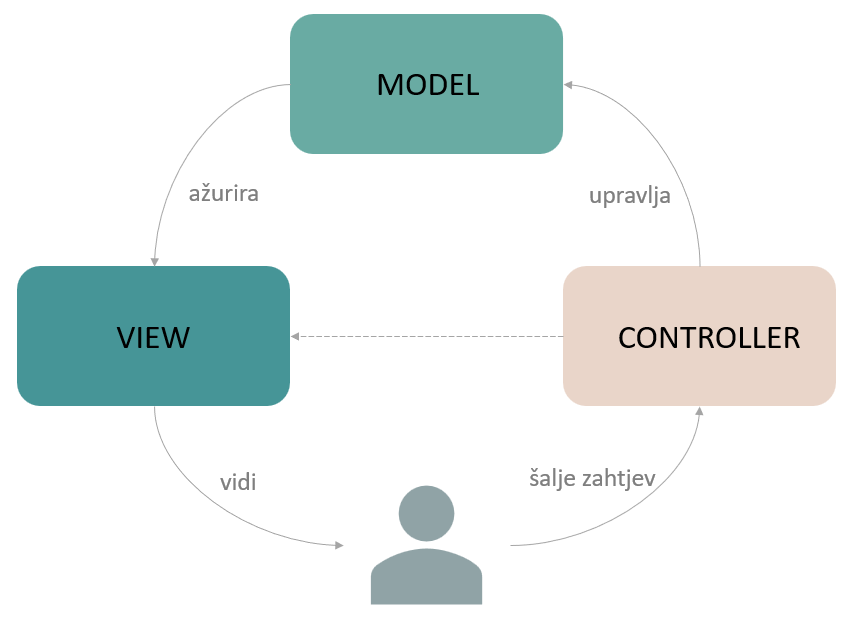
\includegraphics[scale=0.75]{slike/mvc.PNG} %veličina slike u odnosu na originalnu datoteku i pozicija slike
			\centering
			\caption{MVC koncept}
			\label{fig:mvcSkica}
		\end{figure}

		Koncept dijeli aplikaciju na tri sloja – model, view i controller. Svaki sloj izvršava određeni skup zadataka, a svi slojevi djeluju zajedno kako bi ostvarili traženu funkcionalnost aplikacije. Omogućen je nezavisan razvoj pojedinih dijelova čime se pojednostavljuje razvoj i testiranje. 

		\underbar{\textit{Model}} je središnja komponenta ovog koncepta. Upravlja podacima i logikom aplikacije, komunicira s bazom te nema dodira sa sučeljem. Prima zahtjeve od upravljača da se ažurira.

		\underbar{\textit{View}} sadrži komponente aplikacije vidljive korisniku. Omogućuje vizualizaciju podataka spremljenih u modelu i nudi interakciju  korisnikom.

		\underbar{\textit{Controller}}  prima unesene podatke i prevodi ih u naredbe za model i view. Upravlja zahtjevima korisnika i prenosi ih ostalim elementima.
				
		\section{Baza podataka}
			
		 Za potrebe našeg sustava, odabrali smo relacijsku bazu podataka zbog njezine strukture koja olakšava modeliranje stvarnog svijeta. Osnovna građevna jedinica baze je relacija, odnosno tablica koja je identificirana imenom i skupom atributa. Glavna funkcija baze podataka je brza i jednostavna pohrana, izmjena i dohvat podataka za daljnju obradu. Baza podataka naše aplikacije uključuje sljedeće entitete:
		
		\begin{packed_item}
			\item  UserCustom		\textit{~ (korisnik)}
			\item  UserAuth			\textit{~ (prijava za korisnika)}
			\item  Advertisement	\textit{~ (oglas)}
			\item  Pet				\textit{~ (ljubimac)}
			\item  Picture			\textit{~ (slika)}
			\item  Message			\textit{~ (poruka)}
		\end{packed_item}
		
			\subsection{Opis tablica}
			
			
			\textbf{UserCustom}\hspace{10pt}Ovaj entitet sadržava sve važne informacije o korisniku aplikacije.
			Sadrži atribute: id (korisnički identifikacijski broj), username (korisničko ime), isShelter, firstName (ime korisnika), lastName (prezime korisnika), shelterName (ime skloništa ako je riječ o skloništu), email i phoneNumber (broj telefona). Ovaj entitet u vezi je 
			\textit{One-to-One} s entitetom UserAuth preko atributa username (korisničko ime korisnika),
			u vezi \textit{One-to-Many} s Message (poruka) preko korisničkog identifikacijskog broja,
			u vezi \textit{One-to-Many} s entitetom Advertisement preko korisničkog identifikacijskog broja (ili identifikacijskog broja skloništa).
			
				%Svjetlozelenom bojom označite primarni ključ. Svjetlo plavom označite strani ključ
				
				\begin{longtblr}[
					label=none,
					entry=none
					]{
						width = \textwidth,
						colspec={|X[6,l]|X[6, l]|X[20, l]|}, 
						rowhead = 1,
					} %definicija širine tablice, širine stupaca, poravnanje i broja redaka naslova tablice
					\hline \SetCell[c=3]{c}{\textbf{UserCustom}}	 \\ \hline[3pt]
					\SetCell{LightGreen}id & INT	&  jedinstveni brojčani identifikator korisnika	\\ \hline
					username & VARCHAR	&  jedinstveni identifikator korisnika	\\ \hline
					isShelter & BOOLEAN	&  oznaka je li korisnik sklonište	\\ \hline
					firstName & VARCHAR	&  ime korisnika	\\ \hline
					lastName & VARCHAR	&  prezime korisnika	\\ \hline
					shelterName & VARCHAR	&  ime skloništa	\\ \hline
					email & EMAIL \textit{(definirano u bazi podataka)}	&  e-mail adresa korisnika	\\ \hline
					phoneNumber & VARCHAR	&  broj telefona korisnika	\\ \hline
				\end{longtblr}
				
			\textbf{UserAuth}\hspace{10pt}Ovaj entitet sadržava sve što je potrebno kako bi se u sustav prijavio korisnik, a to je njegov username (korisničko ime) i password (pripadajuća loznika).Ovaj entitet je u vezi
			\textit{One-to-One} s entitetom UserCustom preko atributa username (korisničko ime).
			
				\begin{longtblr}[
					label=none,
					entry=none
					]{
						width = \textwidth,
						colspec={|X[6,l]|X[6, l]|X[20, l]|}, 
						rowhead = 1,
					} %definicija širine tablice, širine stupaca, poravnanje i broja redaka naslova tablice
					\hline \SetCell[c=3]{c}{\textbf{UserAuth}}	 \\ \hline[3pt]
					\SetCell{LightBlue}	username & VARCHAR &  jedinstveni identifikator korisnika  	\\ \hline
					password & VARCHAR	&  hash lozinke	\\ \hline
				\end{longtblr}
				
			
			\textbf{Advertisement}\hspace{10pt}Ovaj entitet sadržava sve važne informacije o oglasima koje će korisnici moći postavljati ili čitati.
			Sadrži atribute: id (identifikacijski broj oglasa), category (kategoriju), deleted (podatak o tome je li oglas izbrisan), dateTimeAdv (vrijeme oglašavanja), isInShelter (podatak o tome je li oglas ljubimca označen da je u skloništu), userId (ID korisnika), petId (ID ljubimca) i shelterId (ID skloništa).
			Ovaj entitet je u vezi
			\textit{Many-to-One} s entitetom UserCustom preko atributa userId i shelterId,
			u vezi \textit{One-to-Many} s entitetom Message preko identifikacijskog broja oglasa,
			u vezi \textit{One-to-Many} s entitetom Picture također preko identifikacijskog broja oglasa
			te u vezi \textit{One-to-One} s entitetom Pet (ljubimcem) preko identifikacijskog broja ljubimca.
			
				\begin{longtblr}[
					label=none,
					entry=none
					]{
						width = \textwidth,
						colspec={|X[6,l]|X[6, l]|X[20, l]|}, 
						rowhead = 1,
					} %definicija širine tablice, širine stupaca, poravnanje i broja redaka naslova tablice
					\hline \SetCell[c=3]{c}{\textbf{Advertisement}}	 \\ \hline[3pt]
					\SetCell{LightGreen}	id & INT &  jedinstveni brojčani identifikator oglasa	\\ \hline
					category & ENUM	&  kategorije: lost, found, abandoned, sheltered, dead	\\ \hline
					deleted & BOOLEAN	&  oznaka je li oglas izbrisan	\\ \hline
					dateTimeAdv & TIMESTAMP	&  vrijeme postavljanja oglasa	\\ \hline
					isInShelter & BOOLEAN	&  oznaka je li ljubimac smješten u sklonište	\\ \hline
					\SetCell{LightBlue} userId & INT	&  jedinstveni brojčani identifikator korisnika	\\ \hline
					\SetCell{LightBlue} petId & INT	&  jedinstveni brojčani identifikator ljubimca	\\ \hline
					\SetCell{LightBlue} shelterId & INT	&  jedinstveni brojčani identifikator skloništa	\\ \hline
				\end{longtblr}
				
				
			\textbf{Pet}\hspace{10pt}Ovaj entitet sadržava sve važne informacije o nestalom ljubimcu koje će biti od pomoći pri potrazi.
			Sadrži atribute: id (identifikacijski broj ljubimca), species (vrsta ljubimca), name (ime), color (boja), dateTimeLost (vrijeme kad je ljubimac izgubljen), locationLost (lokacija na kojoj je izgubljen) i description (opis).
			Ovaj entitet je u vezi
			\textit{One-to-One} s entitetom Advertisement  preko atributa identifikacijskog broja ljubimca.
			
				\begin{longtblr}[
					label=none,
					entry=none
					]{
						width = \textwidth,
						colspec={|X[6,l]|X[6, l]|X[20, l]|}, 
						rowhead = 1,
					} %definicija širine tablice, širine stupaca, poravnanje i broja redaka naslova tablice
					\hline \SetCell[c=3]{c}{\textbf{Pet}}	 \\ \hline[3pt]
					\SetCell{LightGreen} id & INT &  jedinstveni brojčani identifikator ljubimca	\\ \hline
					species & ENUM	& vrsta životinje	\\ \hline
					name & VARCHAR	&  ime ljubimca	\\ \hline
					color & VARCHAR	&  boja ljubimca	\\ \hline
					age & INT	&  starost ljubimca	\\ \hline
					dateTimeLost & TIMESTAMP	&  vrijeme kad je ljubimac izgubljen	\\ \hline
					locationLost & VARCHAR	&  opisuje lokaciju na kojoj je ljubimac izgubljen	\\ \hline
					description & TEXT	&  sve dodatne informacije o ljubimcu	\\ \hline
				\end{longtblr}
				
			
			\textbf{Picture}\hspace{10pt}Ovaj entitet omogućava pohranu i korištenje slika koje se koriste pri potrazi za ljubimcima.
			Sadrži atribute: id (identifikacijski broj slike), link, advertId (identifikacijski broj oglasa) i messageId (identifikacijski broj poruke)
			Ovaj entitet je u vezi
			\textit{Many-to-One} s entitetom Advertisement preko atributa identifikacijskog broja ljubimca te je u vezi
			\textit{Many-to-One} s entitetom Message preko ID-a poruke.
			
				\begin{longtblr}[
					label=none,
					entry=none
					]{
						width = \textwidth,
						colspec={|X[6,l]|X[6, l]|X[20, l]|}, 
						rowhead = 1,
					} %definicija širine tablice, širine stupaca, poravnanje i broja redaka naslova tablice
					\hline \SetCell[c=3]{c}{\textbf{Picture}}	 \\ \hline[3pt]
					\SetCell{LightGreen} id & INT &  jedinstveni brojčani identifikator slike	\\ \hline
					link & VARCHAR	& poveznica prema slici	\\ \hline
					\SetCell{LightBlue} advertId & INT	&  jedinstveni brojčani identifikator oglasa \\ \hline
					\SetCell{LightBlue} messageId & INT	&  jedinstveni brojčani identifikator poruke \\ \hline
				\end{longtblr}
				
				
			\textbf{Message}\hspace{10pt}Ovaj entitet sadržava sve važne informacije tijekom komunikacije korisnika prilikom potrage za nestalim ljubimcima.
			Sadrži atribute: id (identifikacijski broj poruke), text, location (lokaciju), dateTimeMess (vrijeme slanja poruke), advertId (ID oglasa) i userId (ID korisnika koji je poslao poruku).
			Ovaj entitet je u vezi
			\textit{Many-to-One} s entitetom UserCustom preko atributa identifikacijskog broja korisnika, u vezi
			\textit{Many-to-One} s entitetom Advertisement preko ID-a oglasa te je u vezi
			\textit{Many-to-One} s entitetom Picture preko identifikacijskog broja poruke.
			
				\begin{longtblr}[
					label=none,
					entry=none
					]{
						width = \textwidth,
						colspec={|X[6,l]|X[6, l]|X[20, l]|}, 
						rowhead = 1,
					} %definicija širine tablice, širine stupaca, poravnanje i broja redaka naslova tablice
					\hline \SetCell[c=3]{c}{\textbf{Message}}	 \\ \hline[3pt]
					\SetCell{LightGreen} id & INT &  jedinstveni brojčani identifikator poruke	\\ \hline
					text & TEXT	& tekstualni dio poruke	\\ \hline
					location & VARCHAR	& lokacija koju korisnik može poslati	\\ \hline
					dateTimeMess & TIMESTAMP	& vrijeme slanja poruke	\\ \hline
					\SetCell{LightBlue} advertId & INT	&  jedinstveni brojčani identifikator oglasa \\ \hline
					\SetCell{LightBlue} userId & INT	&  jedinstveni brojčani identifikator korisnika \\ \hline
				\end{longtblr}
			
			
				
			
			\subsection{Dijagram baze podataka}
				
				%unos slike
				\begin{figure}[H]
					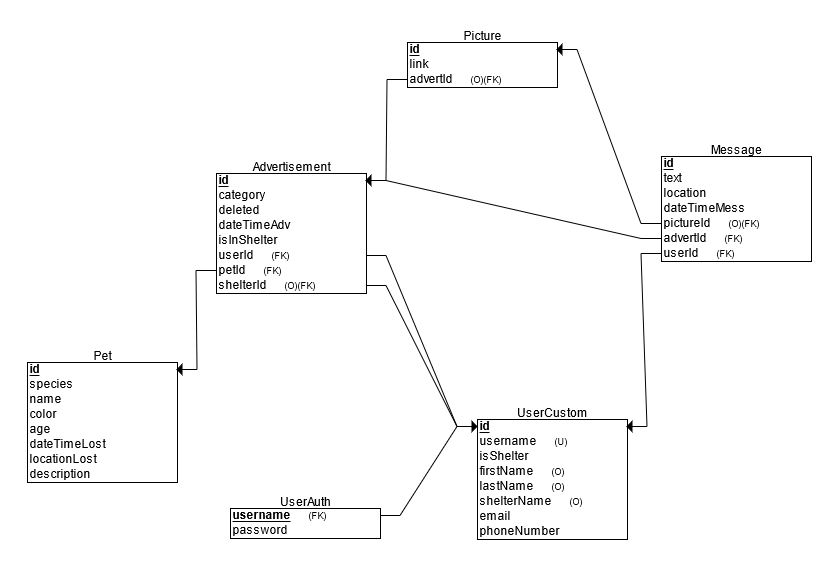
\includegraphics[scale=0.63]{dijagrami/dijagramBaze/relacijskiModel.PNG} %veličina slike u odnosu na originalnu datoteku i pozicija slike
					\centering
					\caption{Relacijski dijagram baze podataka}
					\label{fig:relDijagram}
				\end{figure}

				\begin{figure}[H]
					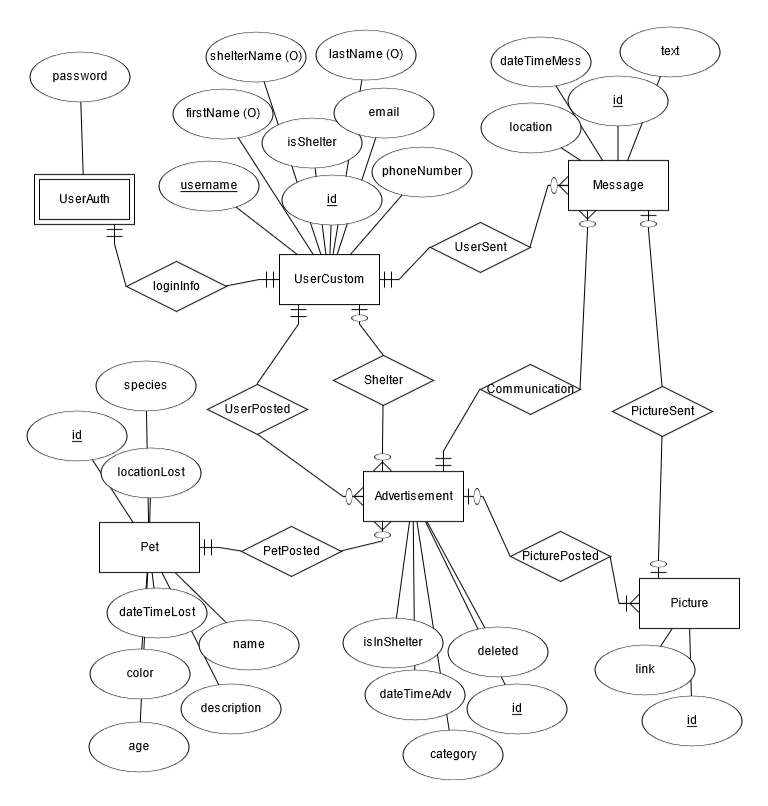
\includegraphics[scale=0.65]{dijagrami/dijagramBaze/ERmodel.PNG} %veličina slike u odnosu na originalnu datoteku i pozicija slike
					\centering
					\caption{E-R dijagram baze podataka}
					\label{fig:erDijagram}
				\end{figure}

			\eject
			
			
		\section{Dijagram razreda}
		
			Na slikama \ref{fig:drModels}, \ref{fig:drDataTransferObjects}, \ref{fig:drRepository} i \ref{fig:drControllers} su prikazani razredi koji pripadaju \textit{backend} dijelu MVC arhitekture. Na slici \ref{fig:drView} prikazani su razredi \textit{frontend} dijela arhitekture. Razredi prikazani na slici \ref{fig:drRepository} prikazuju \textit{Repository} koji je zadužen za interakciju s bazom. Razredi na slici \ref{fig:drControllers} nasljeđuju razred \textit{APIRouter}. Metode implementirane u tim razredima manipuliraju s DTO \textit{(Data transfer object)}, a oni su dohvaćeni pomoću metoda implementiranih u Model razredima.

			Zbog lakše organizacije, razredi su podijeljeni logički po pravu pristupa metodama određenih aktora. Prikazane su isključivo ovisnosti između razreda koji pripadaju istom dijelu dijagrama. Ostale ovisnosti mogu se zaključiti iz naziva i tipova atributa u razredima.

			\begin{figure}[H]
				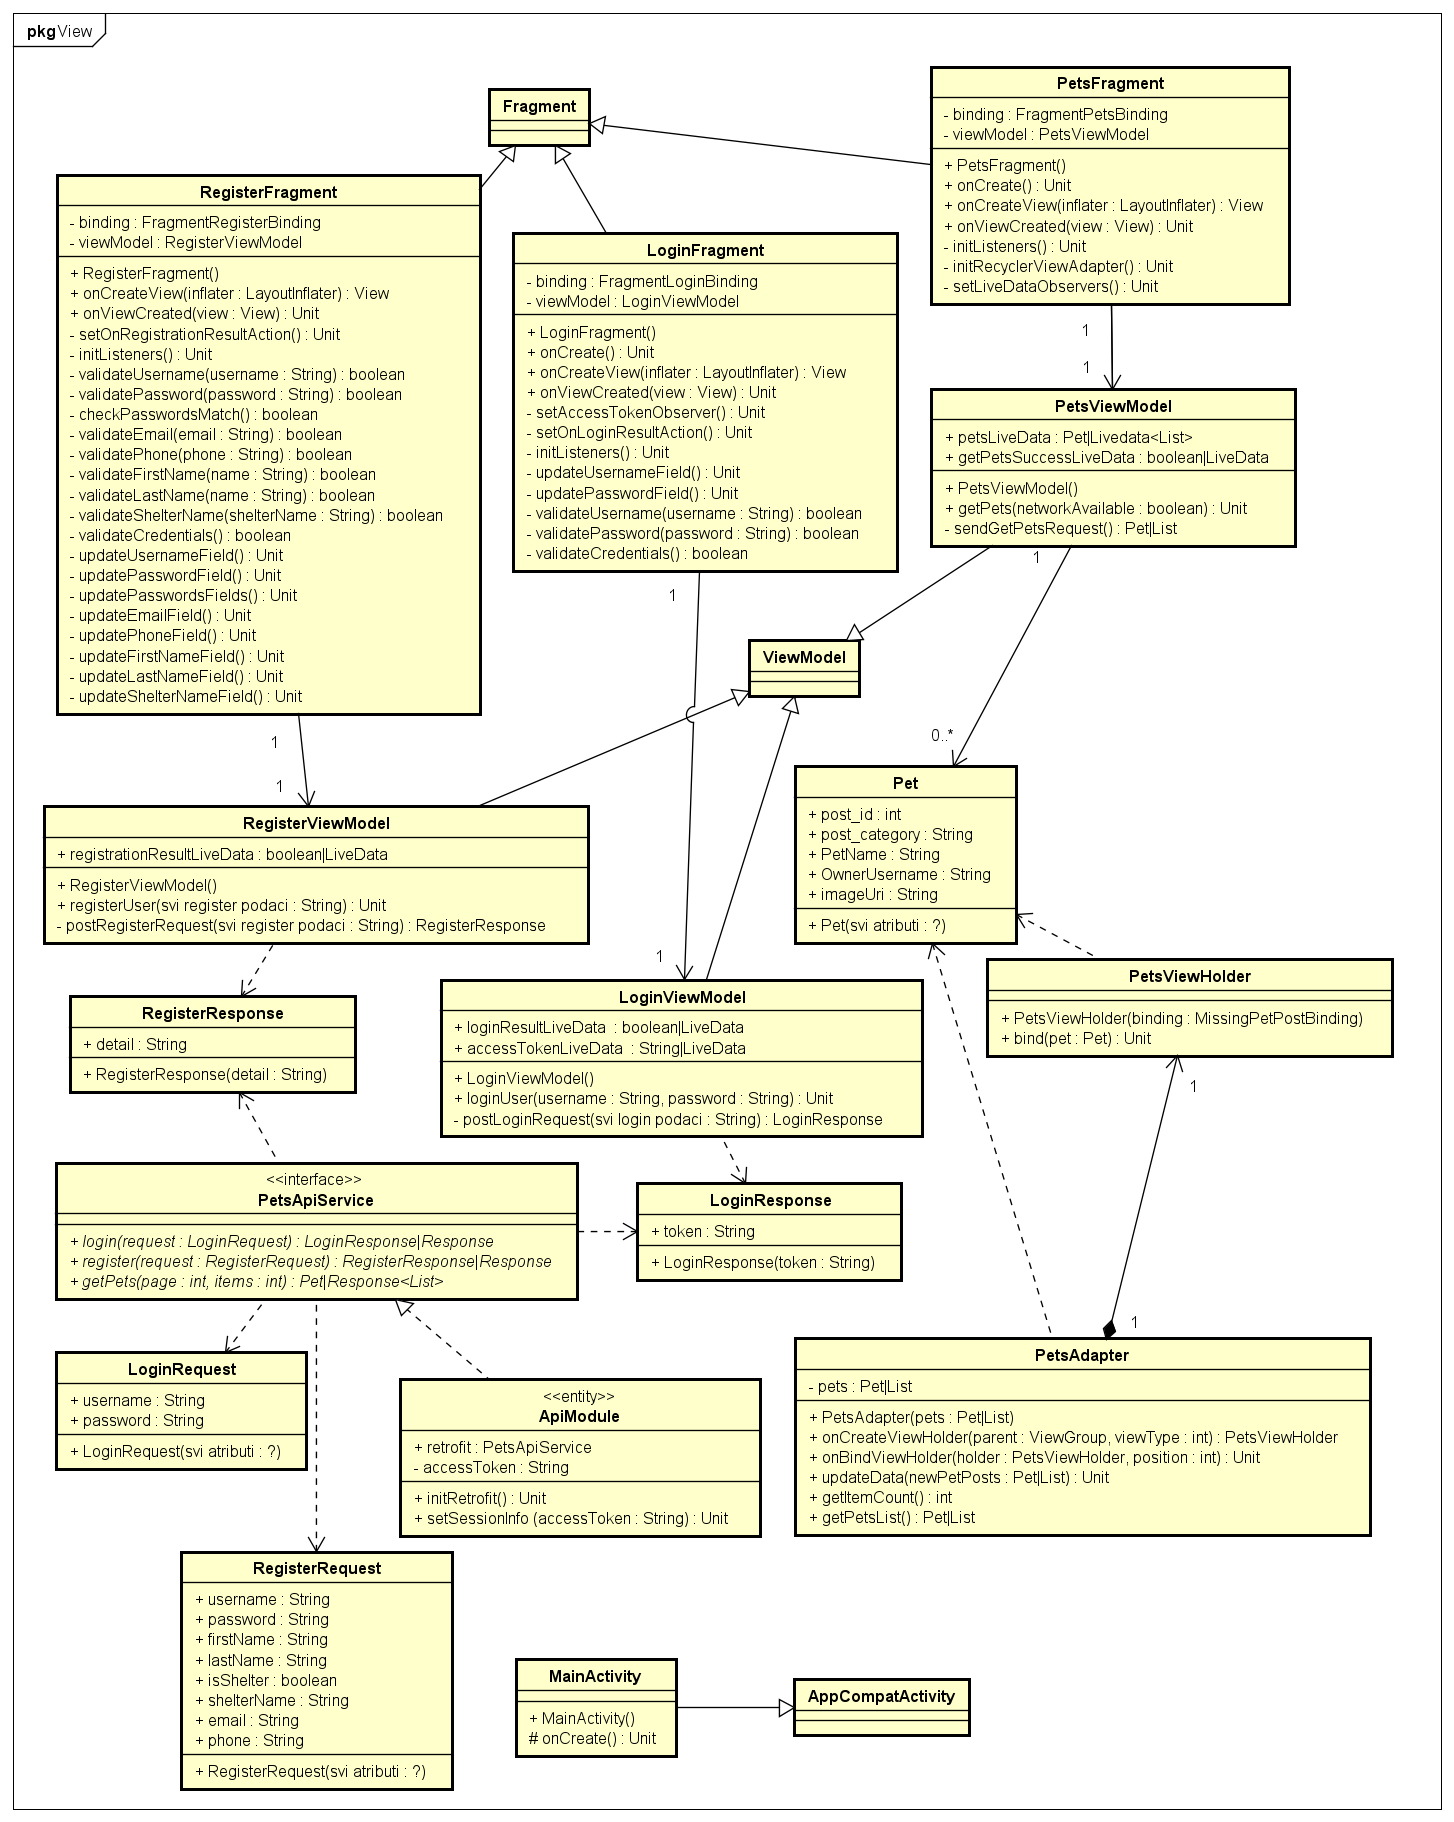
\includegraphics[scale=0.45]{dijagrami/dijagramiRazreda/View.PNG} %veličina slike u odnosu na originalnu datoteku i pozicija slike
				\centering
				\caption{Dijagram razreda - dio View}
				\label{fig:drView}
			\end{figure}

			Model razredi preslikavaju strukturu baze podataka u aplikaciji. Implementirane metode direktno komuniciraju s bazom podataka te vraćaju tražene podatke. Razred UserCustom predstavlja registriranog korisnika koji ima pristup svim stavkama aplikacije. Razred UserAuth predstavlja podatke za prijavu registriranog korisnika. Razred Advertisement predstavlja objavljeni oglas. Pet je razred koji sadrži unesene podatke o nestalom ljubimcu. Razred message predstavlja poruke vezane za komunikaciju o potrazi. Razred Picture predstavlja sliku koja se nalazi ili u oglasu ili u poruci. PetSpecies je enumeracija s mogućim vrstama ljubimca, a AdvertisementCategory enumeracija s kategorijama oglasa.

			\begin{figure}[H]
				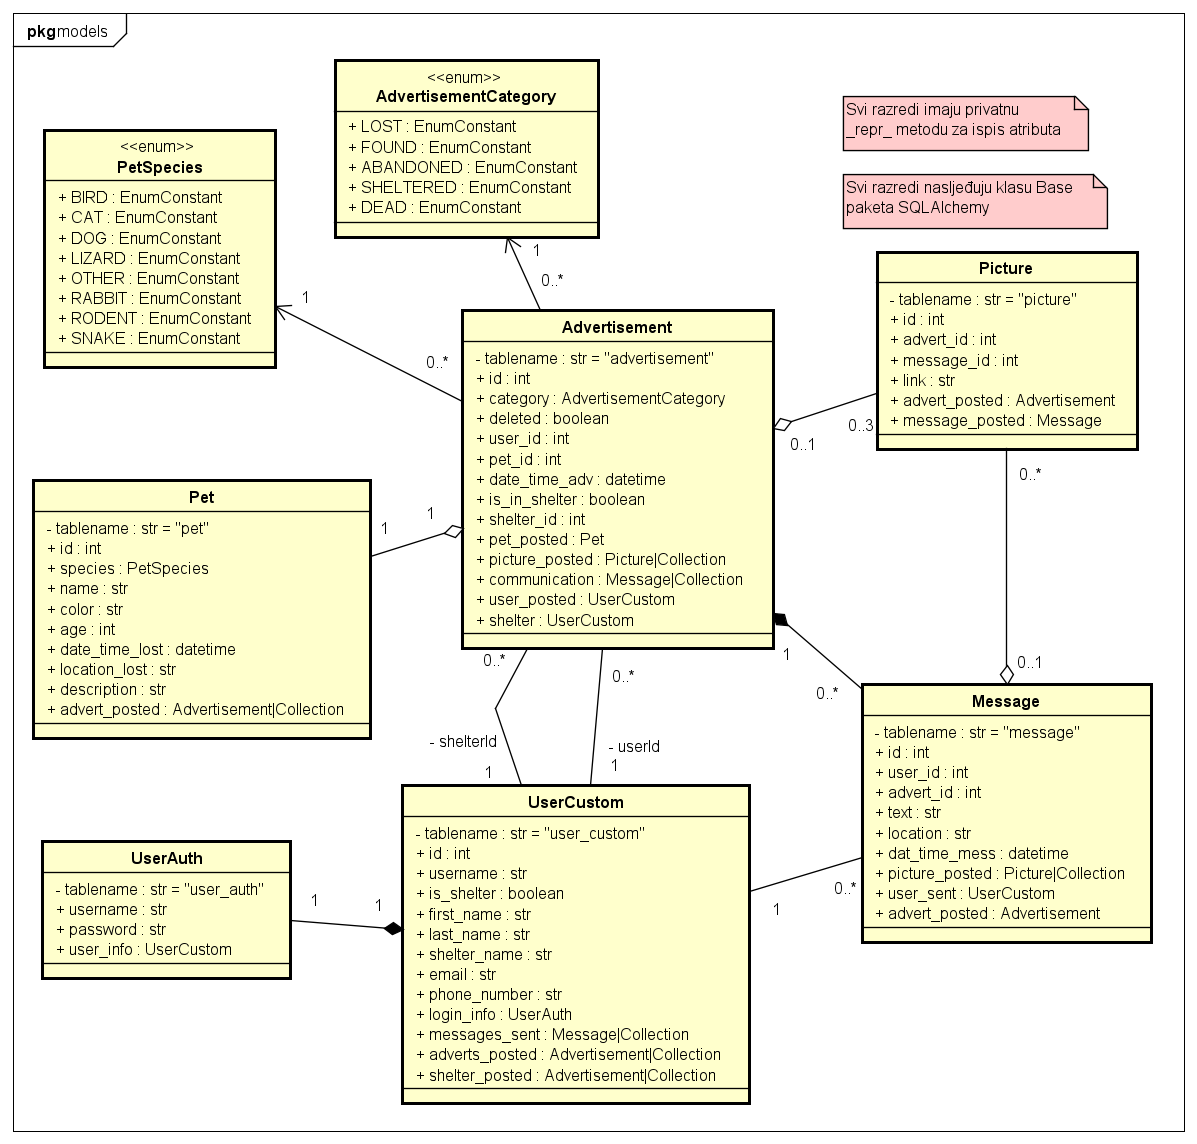
\includegraphics[scale=0.55]{dijagrami/dijagramiRazreda/Models.PNG} %veličina slike u odnosu na originalnu datoteku i pozicija slike
				\centering
				\caption{Dijagram razreda - dio Models}
				\label{fig:drModels}
			\end{figure}
			
			\begin{figure}[H]
				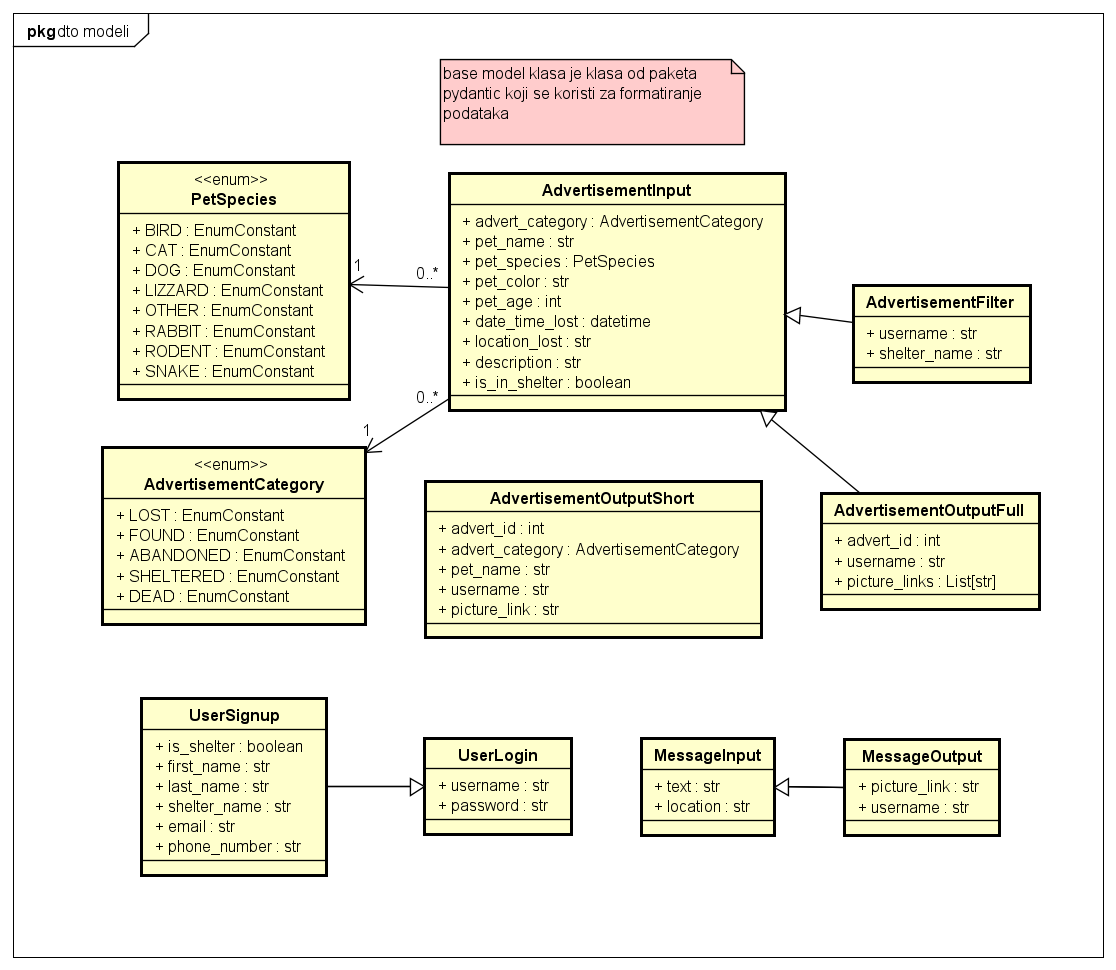
\includegraphics[scale=0.55]{dijagrami/dijagramiRazreda/dto.PNG} %veličina slike u odnosu na originalnu datoteku i pozicija slike
				\centering
				\caption{Dijagram razreda - dio Data transfer objects}
				\label{fig:drDataTransferObjects}
			\end{figure}
			
			\begin{figure}[H]
				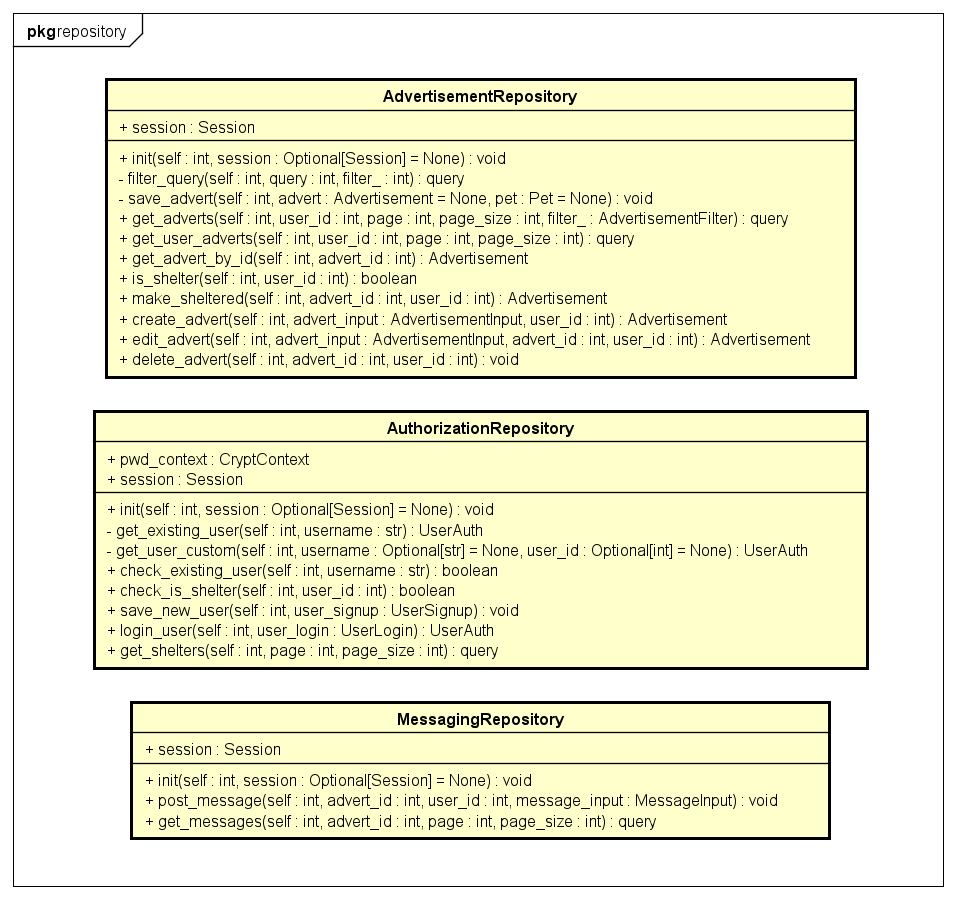
\includegraphics[scale=0.6]{dijagrami/dijagramiRazreda/repo.PNG} %veličina slike u odnosu na originalnu datoteku i pozicija slike
				\centering
				\caption{Dijagram razreda - dio Repository}
				\label{fig:drRepository}
			\end{figure}

			\begin{figure}[H]
				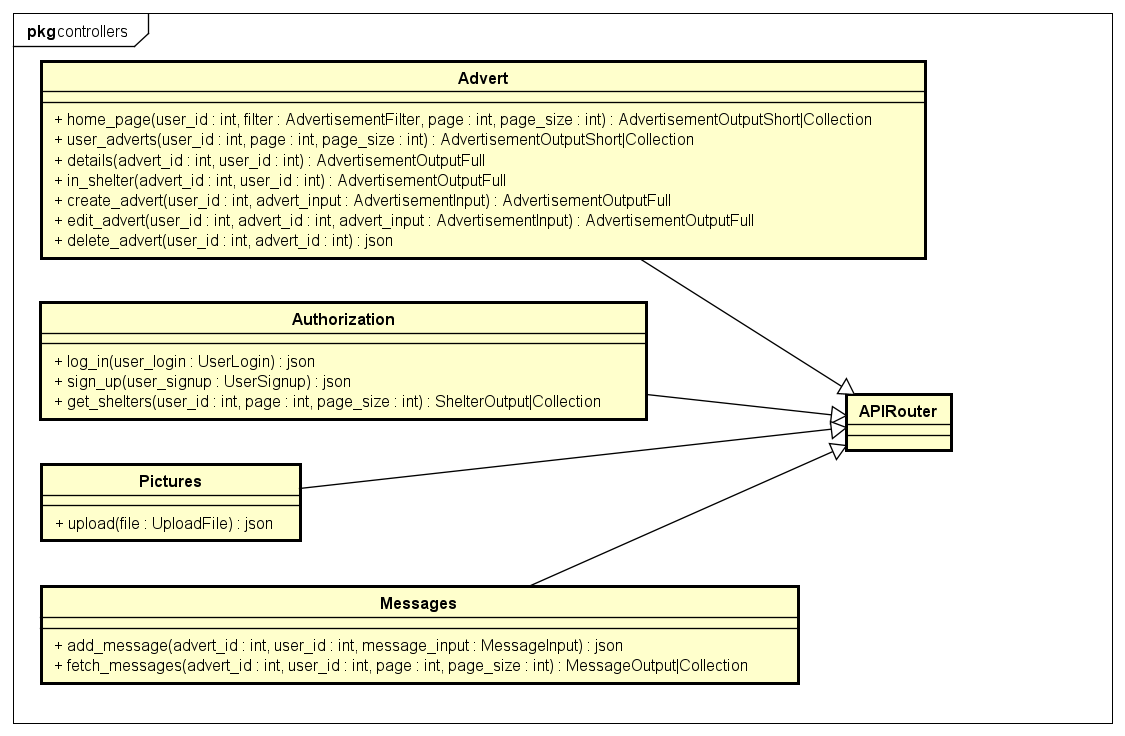
\includegraphics[scale=0.6]{dijagrami/dijagramiRazreda/Controllers.PNG} %veličina slike u odnosu na originalnu datoteku i pozicija slike
				\centering
				\caption{Dijagram razreda - dio Controllers}
				\label{fig:drControllers}
			\end{figure}
			
			\eject
		
		\section{Dijagram stanja}
			
			
			\textbf{\textit{dio 2. revizije}}\\
			
			...
			
			
			\eject 
		
		\section{Dijagram aktivnosti}

			UML-dijagrami aktivnosti su ponašajni UML-dijagrami koji se upotrebljavaju za modeliranje i vizualizaciju dinamičkog ponašanja sustava. Prikazuju tijek aktivnosti, akcija i odluka procesa u sustavu. Svaki novi korak ovisi o završetku i rezultatu prethodnog. Na dijagramu \ref{fig:dAktivnosti} prikazan je proces kreiranja novog oglasa za nestalog ljubimca. Korisnik se prvo prijavljuje u sustav, a zatim odabire opciju za objavu novog oglasa. Unosi željene podatke o ljubimcu koji se onda provjeravaju u aplikaciji i na bazi. Ako su neispravni aplikacija traži ponovni unos, inače se spremaju u bazu. Novi oglas se zatim prikazuje korisniku.
			
			\begin{figure}[H]
				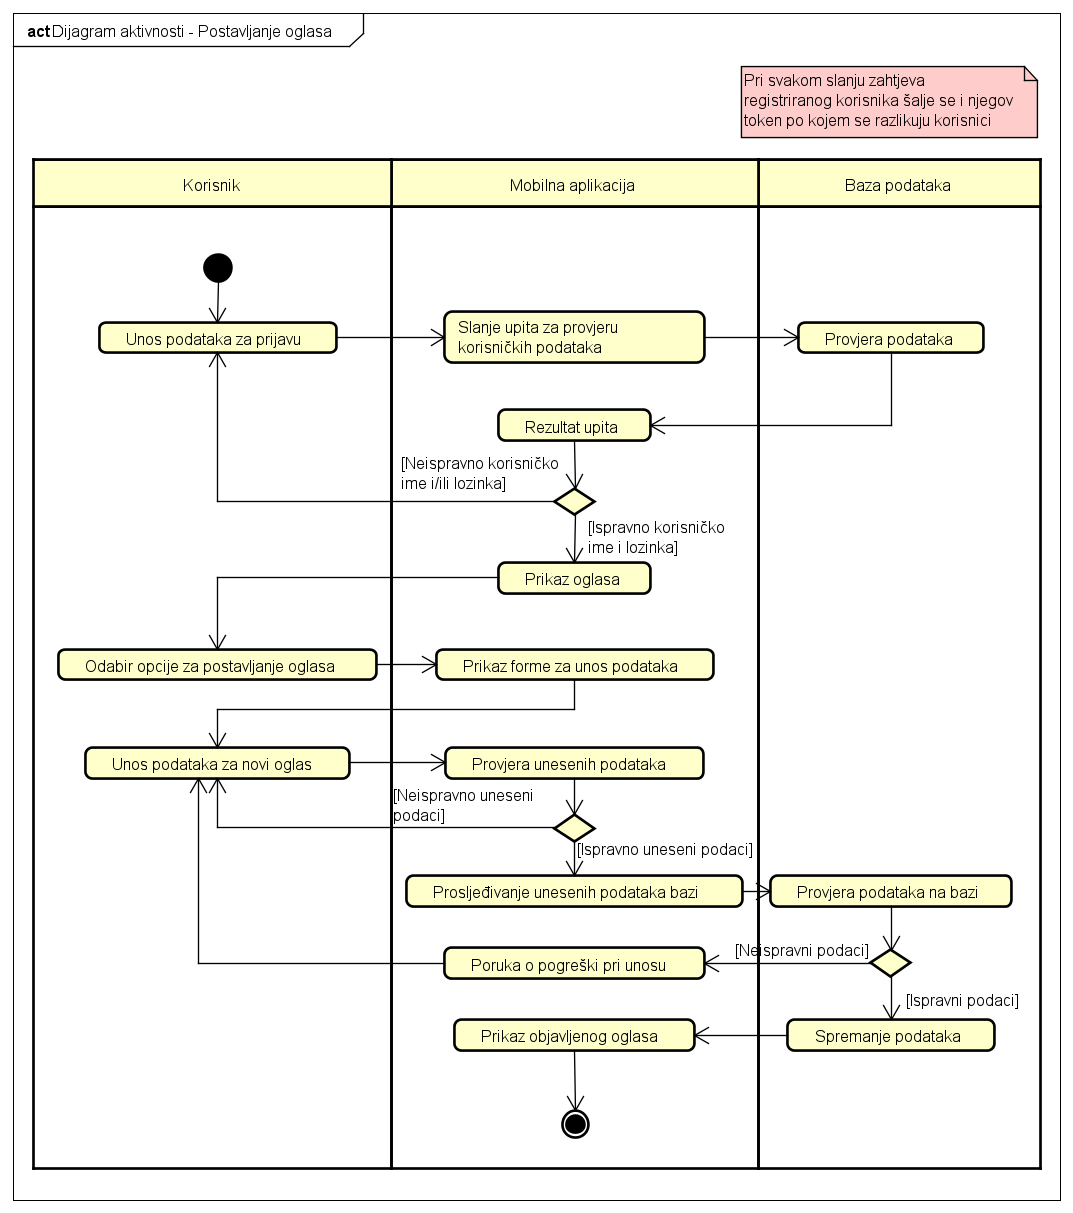
\includegraphics[scale=0.6]{dijagrami/dijagramAktivnosti/dAktivnosti.PNG} %veličina slike u odnosu na originalnu datoteku i pozicija slike
				\centering
				\caption{Dijagram aktivnosti - Postavljanje oglasa}
				\label{fig:dAktivnosti}
			\end{figure}
			
			\eject
		\section{Dijagram komponenti}
		
			\textbf{\textit{dio 2. revizije}}\\
		
			...
	\chapter{Implementacija i korisničko sučelje}
		
		
		\section{Korištene tehnologije i alati}
		
			Komunikacija unutar tima realizirana je korištenjem aplikacija \underline{WhatsApp}\footnote{\url{https://www.whatsapp.com/}} i \underline{Discord}\footnote{\url{https://discord.com/}}. Za izradu UML dijagrama korišten je alat \underline{Astah Professional}\footnote{\url{https://astah.net/}}. Kao sustav za upravljanje izvornim kodom upotrebljavali smo \underline{Git}\footnote{\url{https://git-scm.com/}}, a udaljeni repozitorij projekta je dostupan na web platformi \underline{GitHub}\footnote{\url{https://github.com/}}.

			Kao razvojna okruženja korišteni su \underline{Android Studio}\footnote{\url{https://developer.android.com/studio}} i \underline{PyCharm}\footnote{\url{https://www.jetbrains.com/pycharm/}}. Android Studio je integrirano razvojno okruženje za Googleov operativni sustav Android, izgrađeno na JetBrainsovom IntelliJ IDEA softveru i dizajnirano posebno za Android razvoj. Dostupan je za preuzimanje na Windows, macOS i Linux operativnim sustavima. PyCharm  je integrirano razvojno okruženje koje se koristi za programiranje u Pythonu koji je razvila tvrtka JetBrains. Omogućuje analizu koda, integrirani tester jedinica \textit{(engl. unit testing)}, grafički \textit{debugger} i podržava web razvoj s Djangom. Isto kao i Android Studio, dostupan je na različitim operacijskim sustavima.

			Aplikacija je napisana koristeći radni okvir \underline{FastAPI}\footnote{\url{https://fastapi.tiangolo.com/}} i jezik \underline{Python}\footnote{\url{https://www.python.org/}} za izradu \textit{backenda} te jezik \underline{Kotlin}\footnote{\url{https://kotlinlang.org/}} za izradu \textit{frontenda}. FastAPI je moderan web okvir za izgradnju RESTful API-ja u Pythonu. Popularan je među programerima zbog svoje jednostavnosti, robusnosti i brzine.

			Baza podataka se nalazi na poslužitelju u \underline{Renderu}\footnote{\url{https://render.com/}}. To je objedinjeni oblak za izradu i pokretanje svih aplikacija i web stranica s besplatnim TLS certifikatima, globalnim CDN-om, privatnim mrežama i automatskim deploymentom iz Gita.
			
			\eject 
		
	
		\section{Ispitivanje programskog rješenja}
			
			Ispitivanje aplikacije provelo se na strukturiran način pomoću unit testova na \textit{backendu} i ????????? na \textit{frontendu}. Aplikaciju smo ispitali po obrascima uporabe kako bi provjerili svu osnovnu funkcionalnost aplikacije, kao i nasumičnim kretanjem po aplikaciji kako bi otkrili moguća nepredviđena ponašanja i ispravili neočekivane greške. Ispitan je cijeli sustav, no zbog jednostavnosti dokumentacije ovdje će biti prikazan samo dio testova.
			
			\subsection{Ispitivanje komponenti}
		
			Proveli smo ispitivanje jedinica (engl. \textit{unit testing}) nad razredima koji implementiraju osnovne funkcionalnosti. U nastavku će biti prikazan izvorni kod i prikaz rezultata izvođenja ispita u razvojnom okruženju.

			Za konfiguraciju i provođenje svih testova bile su nam potrebne sljedeće funkcije: 
	
			\begin{packed_item}
			
				\item pytest{\_}configure - stvara testnu bazu na lokalnom poslužitelju prije testiranja
				\item pytest{\_}unconfigure - \textit{dropa} lokalnu tekstnu bazu nakon završetka testiranja
				\item pytest fixture test{\_}session - da testovi nebi utjecali jedan na drugog, za svakog stvori izoliranu okolinu
				\item mock{\_}user{\_}token - dependency override za provjeru tokena na endpointima, token se provjerava zasebno
				\item user{\_}factory - direktno stvara usera na bazi
				\item advert{\_}factory - direktno stvara advert na bazi
			
			\end{packed_item}

			Izvorni kod navedenih funkcija priložen je u nastavku.
			\begin{lstlisting}[language=Python]
def pytest_configure():
    create_database(
        URL.create(
            "postgresql",
            username=settings.POSTGRES_USER,
            password=settings.POSTGRES_PASSWORD,
            host=settings.POSTGRES_HOST,
            port=settings.POSTGRES_PORT,
            database=settings.TEST_DATABASE,
        )
    )

def pytest_unconfigure():
    drop_database(
        URL.create(
            "postgresql",
            username=settings.POSTGRES_USER,
            password=settings.POSTGRES_PASSWORD,
            host=settings.POSTGRES_HOST,
            port=settings.POSTGRES_PORT,
            database=settings.TEST_DATABASE,
        )
    )

@pytest.fixture(scope="function")
def test_session():
    EngineManager.set_database(settings.TEST_DATABASE)
    engine = EngineManager.get_engine()
    Base.metadata.create_all(engine)

    test_session_mold = sessionmaker(bind=engine, expire_on_commit=False)
    test_session = test_session_mold()
    yield test_session

    Base.metadata.drop_all(engine)
    EngineManager.unset_database()

def mock_user_token():
    return 1

def user_factory(user_id: int, session: Session):
    user = (
        UserCustom(
                id=user_id,
                username=('test_username_' + str(user_id)),
                is_shelter=False,
                email='test_email',
                phone_number='test_number'
        )
    )
    user_auth = UserAuth(username=('test_username_' + str(user_id)), password='1234')
    session.add(user)
    session.add(user_auth)
    session.commit()
    return user

def advert_factory(id: int, user_id: int, session: Session):
    pet = Pet(
        id=id,
        name=('test_pet_' + str(id)),
        location_lost=('test_location_' + str(id)),
    )
    advert = Advertisement(
        id=id,
        pet_id=id,
        user_id=user_id,
        category='lost'
    )
    session.add(pet)
    session.add(advert)
    session.commit()
			\end{lstlisting}

			U nastavku je naveden dio testova koje smo proveli.

			Klasa \textit{TestAuthentication} provodi dva testa. Prvi test ispitao je generiranje i dekodiranje korisničkog tokena. Drugi test ispitao je funkcionalnost prijave i registracije korisnika pri ulasku u aplikaciju. Komponenta je prošla testove i rezultat ispitivanja prikazan je na slici \ref{fig:test1i2}. Izvorni kod za ova dva testa je sljedeći: 
			\begin{lstlisting}
class TestAuthentication:

    def test_auth_utils(self, test_session):
        user = user_factory(1, test_session)
        token = generate_token(user)
        assert len(token) == 181

        decoded = validate_token(token)
        assert decoded == user.id

    def test_signup_and_login(self, test_session):
        with TestClient(app) as client:
            result_signup = client.post(
                "/api/authorization/signup",
                json={
                    "username": "test_shelter",
                    "password": "password",
                    "is_shelter": True,
                    "shelter_name": "Test Shelter",
                    "email": "test@shelter.com",
                    "phone_number": "111"
                }
            )

            assert result_signup.status_code == 201
            assert result_signup.json().get("detail") == "User successfully saved"

            result_login = client.post(
                "/api/authorization/login",
                json={
                    "username": "test_shelter",
                    "password": "password"
                }
            )

            assert result_login.status_code == 200
            assert result_login.json().get("token") is not None
            assert result_login.json().get("is_shelter")
            assert result_login.json().get("current_user_username") == "test_shelter"
			\end{lstlisting}

			\begin{figure}[H]
			 	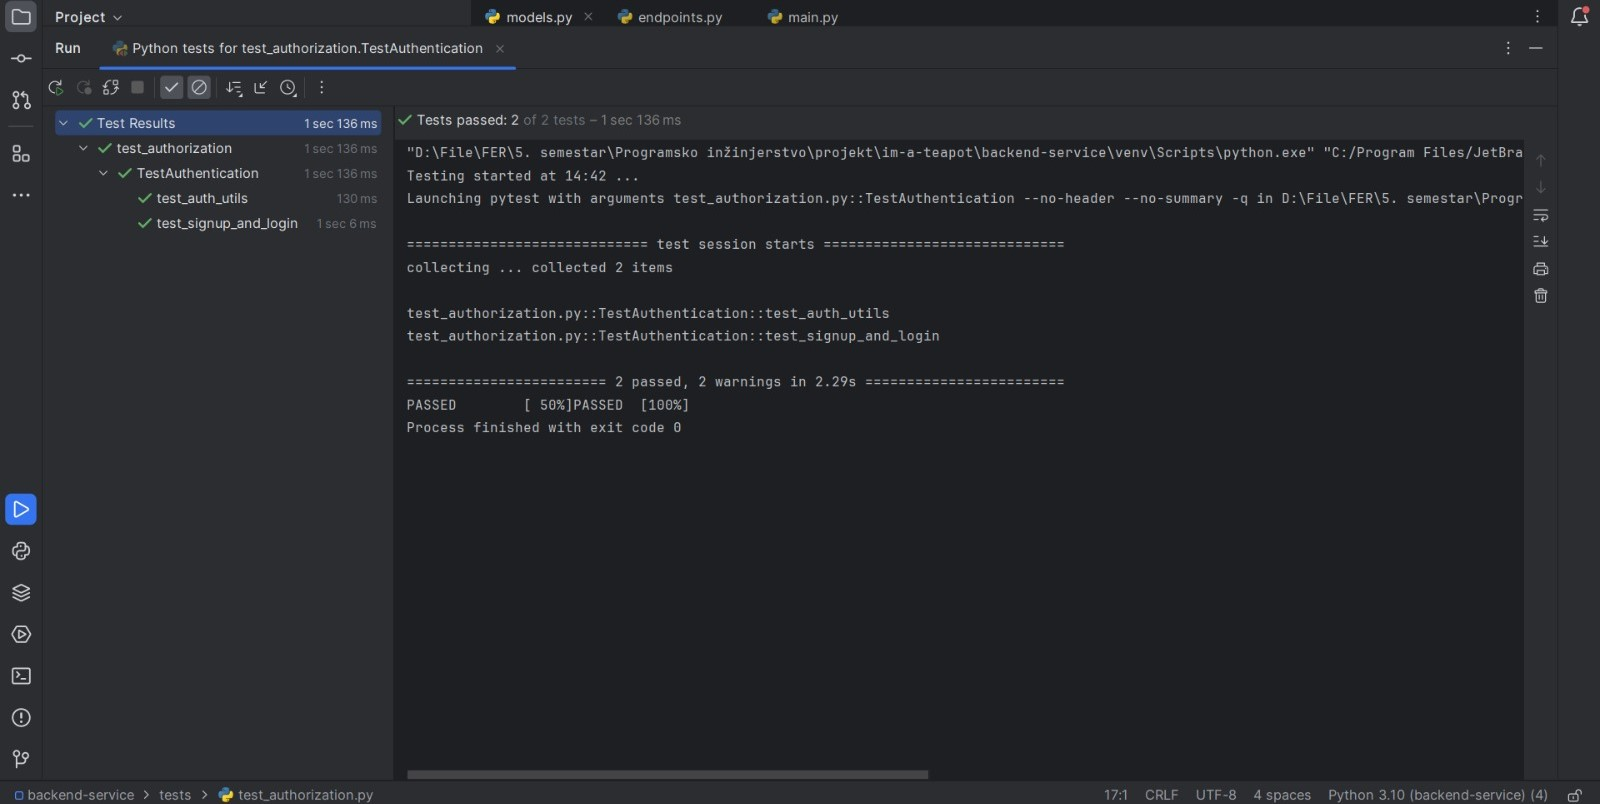
\includegraphics[scale=0.42]{slike/test1i2.jpg} %veličina slike u odnosu na originalnu datoteku i pozicija slike
			 	\centering
			 	\caption{Rezultati testa 1. i testa 2.}
			 	\label{fig:test1i2}
			 \end{figure}

			Klasa \textit{TestMessaging} provjerava slanje i dohvaćanje poruka o nestalom ljubimcu. Komponenta je prošla test i rezultat ispitivanja prikazan je na slici \ref{fig:test3}. Izvorni kod testa je sljedeći:
			\begin{lstlisting}
class TestMessaging:

    def test_add_and_fetch_message(self, test_session):
        app.dependency_overrides[validate_token] = mock_user_token
        user_factory(1, test_session)
        user_factory(2, test_session)
        advert_factory(1, 1, test_session)

        with TestClient(app) as client:
            result = client.post(
                "/api/messages/1/add",
                json={
                    "text": "message_1"
                }
            )
            assert result.status_code == 200

            client.post(
                "/api/messages/1/add",
                json={
                    "text": "message_2"
                }
            )
            assert result.status_code == 200

            result = client.get(
                "/api/messages/1"
            )
            assert result.status_code == 200
            assert len(result.json()) == 2
			\end{lstlisting}

			\begin{figure}[H]
			 	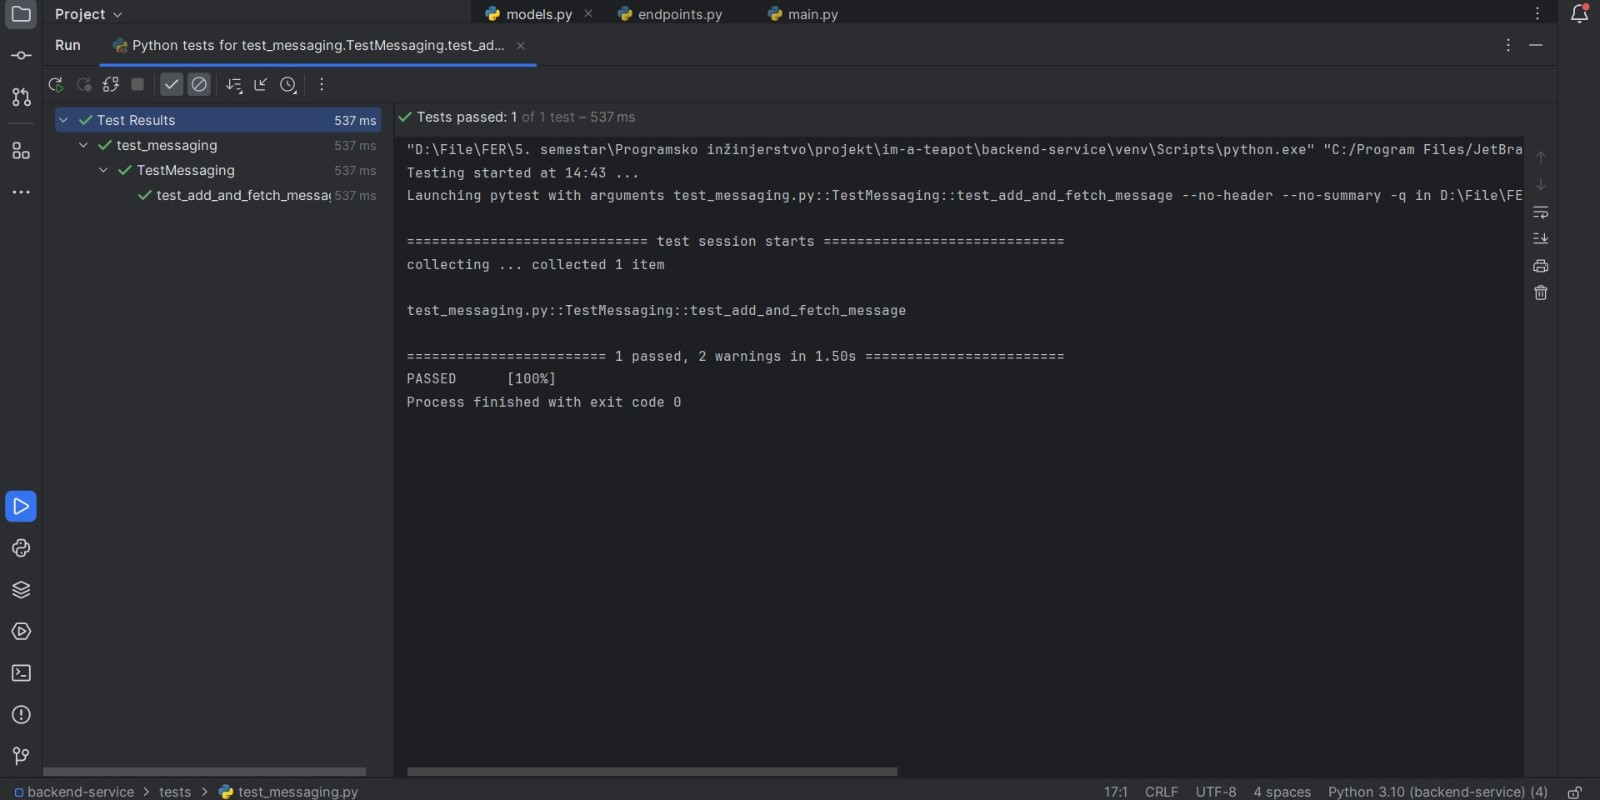
\includegraphics[scale=0.42]{slike/test3.jpg} %veličina slike u odnosu na originalnu datoteku i pozicija slike
			 	\centering
			 	\caption{Rezultati testa 3.}
			 	\label{fig:test3}
			 \end{figure}

			Klasa \textit{TestAdvertActions} izvodi tri testa nad oglasima o nestalim ljubimcima. Ispitala je postavljanje, izmjenu i brisanje oglasa. Komponenta aplikacije je prošla sva tri testa i rezultati su prikazani na slici \ref{fig:test4i5i6}. Izvorni kod ovih testova je sljedeći:
			\begin{lstlisting}
class TestAdvertActions:

    def test_create(self, test_session):
        app.dependency_overrides[validate_token] = mock_user_token
        user_factory(1, test_session)
        with TestClient(app) as client:
            result = client.post(
                "/api/advert/create",
                json={
                    "pet_name": "Edgar",
                }
            )
            assert result.status_code == 200

    def test_edit(self, test_session):
        app.dependency_overrides[validate_token] = mock_user_token
        user_factory(1, test_session)
        advert_factory(1, 1, test_session)
        with TestClient(app) as client:
            result = client.put(
                "/api/advert/1/edit",
                json={
                    "pet_name": "Allan",
                }
            )
            assert result.status_code == 200
            assert result.json().get("pet_name") == "Allan"

    def test_delete(self, test_session):
        app.dependency_overrides[validate_token] = mock_user_token
        user_factory(1, test_session)
        advert_factory(1, 1, test_session)
        with TestClient(app) as client:
            result = client.delete(
                "/api/advert/1/delete"
            )
            assert result.status_code == 200
			\end{lstlisting}

			\begin{figure}[H]
			 	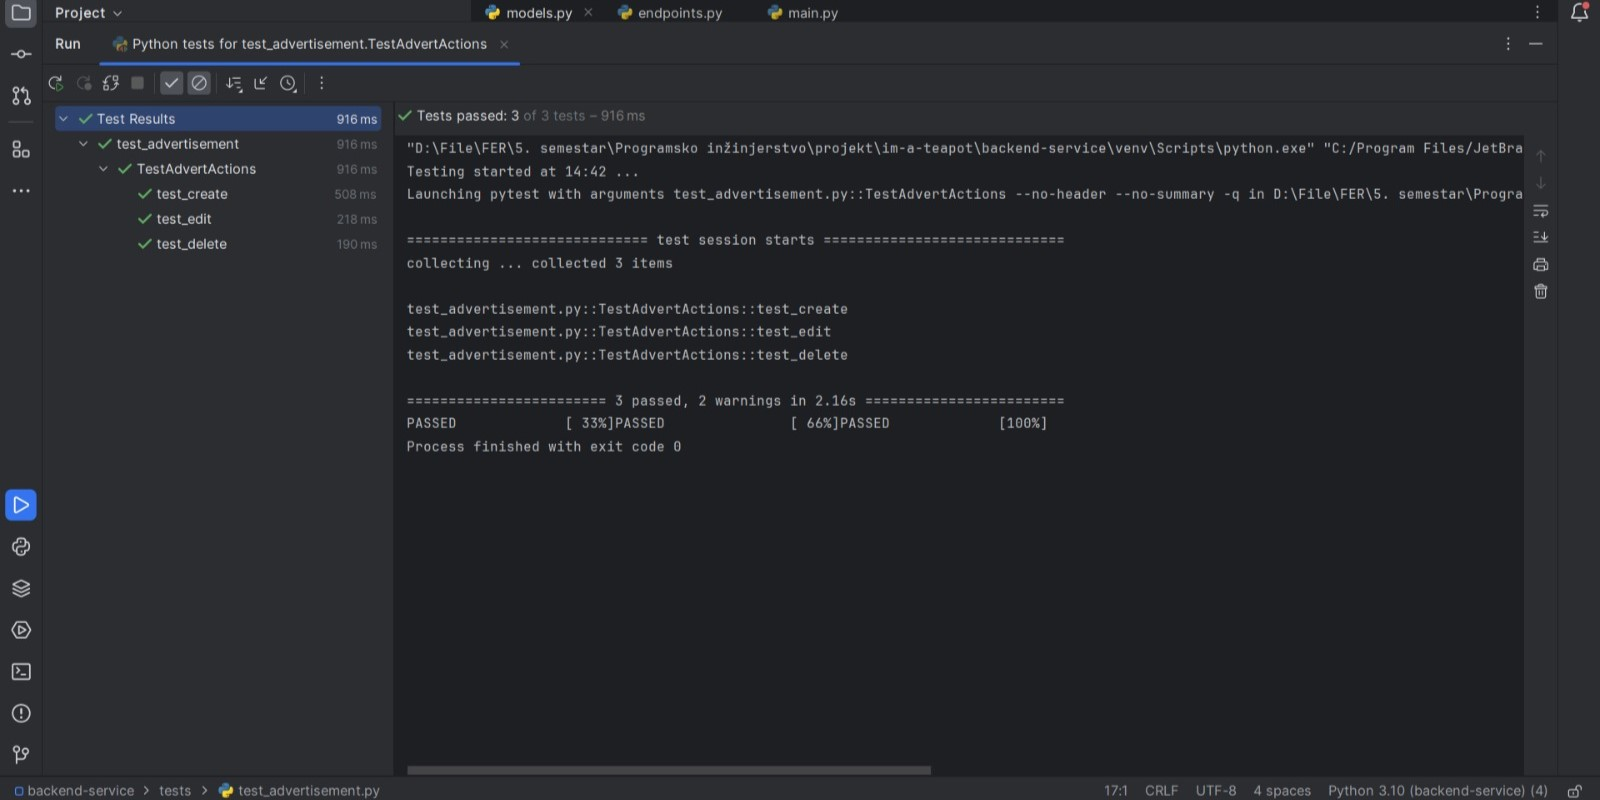
\includegraphics[scale=0.42]{slike/test4i5i6.jpg} %veličina slike u odnosu na originalnu datoteku i pozicija slike
			 	\centering
			 	\caption{Rezultati testa 4., testa 5. i testa 6.}
			 	\label{fig:test4i5i6}
			 \end{figure}

			Klasa \textit{TestHome} provodi dva testa. Prvi je ispitivanje pretraživanja po imenu ljubimca i po korisničkom imenu. Komponenta je prošla ovaj test, a rezultat ispitivanja prikazan je na slici \ref{fig:test7}. Druga stvar koju ova klasa ispituje je pretraživanje po lokaciji. Ta funkcionalnost nije implementirana u našoj aplikaciji, pa zato komponenta pada na ovom testu. Rezultat je prikazan na slikama \ref{fig:test8a} i \ref{fig:test8b}. Izvorni kod klase koja provodi ova ispitivanja prikazan je u nastavku.
			\begin{lstlisting}
class TestHome:

    def test_filter__by_pet_name_and_username(self, test_session):
        user_factory(1, test_session)
        user_factory(2, test_session)
        advert_factory(1, 1, test_session)
        advert_factory(2, 2, test_session)

        with TestClient(app) as client:
            result = client.get(
                "/api/advert/",
                params={"pet_name": "test_pet_1", "username": "test_username_1"}
            )

            assert result.status_code == 200
            assert len(result.json()) == 1

    def test_filter__by_location(self, test_session):
        user_factory(1, test_session)
        user_factory(2, test_session)
        advert_factory(1, 1, test_session)
        advert_factory(2, 2, test_session)

        with TestClient(app) as client:
            result = client.get(
                "/api/advert/",
                params={"location_lost": "test_location_1"}
            )

            assert result.status_code == 200
            assert len(result.json()) == 1
			\end{lstlisting}

			\begin{figure}[H]
			 	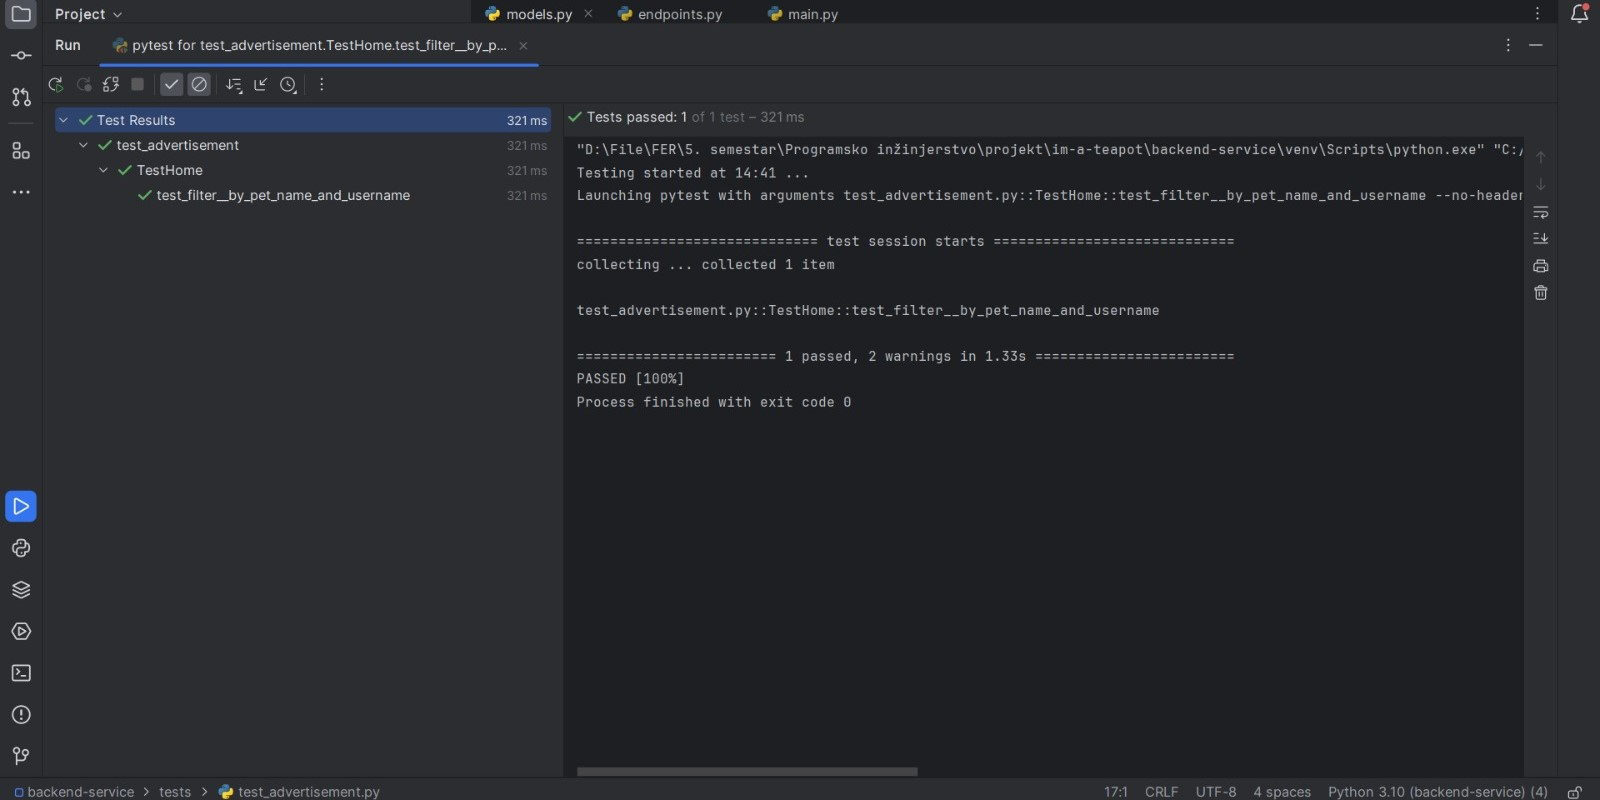
\includegraphics[scale=0.42]{slike/test7.jpg} %veličina slike u odnosu na originalnu datoteku i pozicija slike
			 	\centering
			 	\caption{Rezultati testa 7.}
			 	\label{fig:test7}
			 \end{figure}

			\begin{figure}[H]
			 	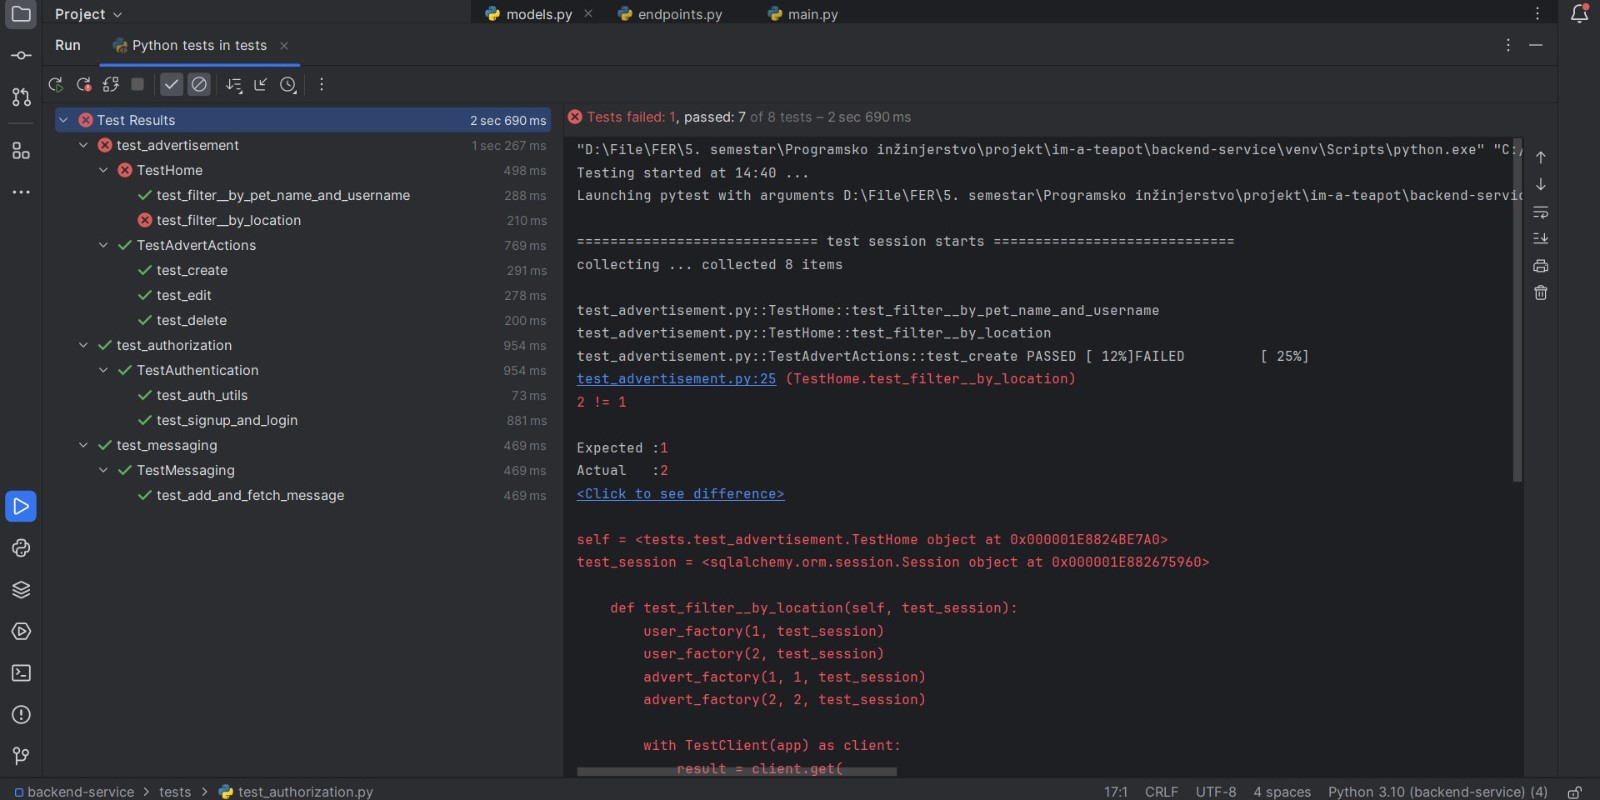
\includegraphics[scale=0.42]{slike/test8a.jpg} %veličina slike u odnosu na originalnu datoteku i pozicija slike
			 	\centering
			 	\caption{Rezultati testa 8. - 1. dio}
			 	\label{fig:test8a}
			 \end{figure}

			\begin{figure}[H]
			 	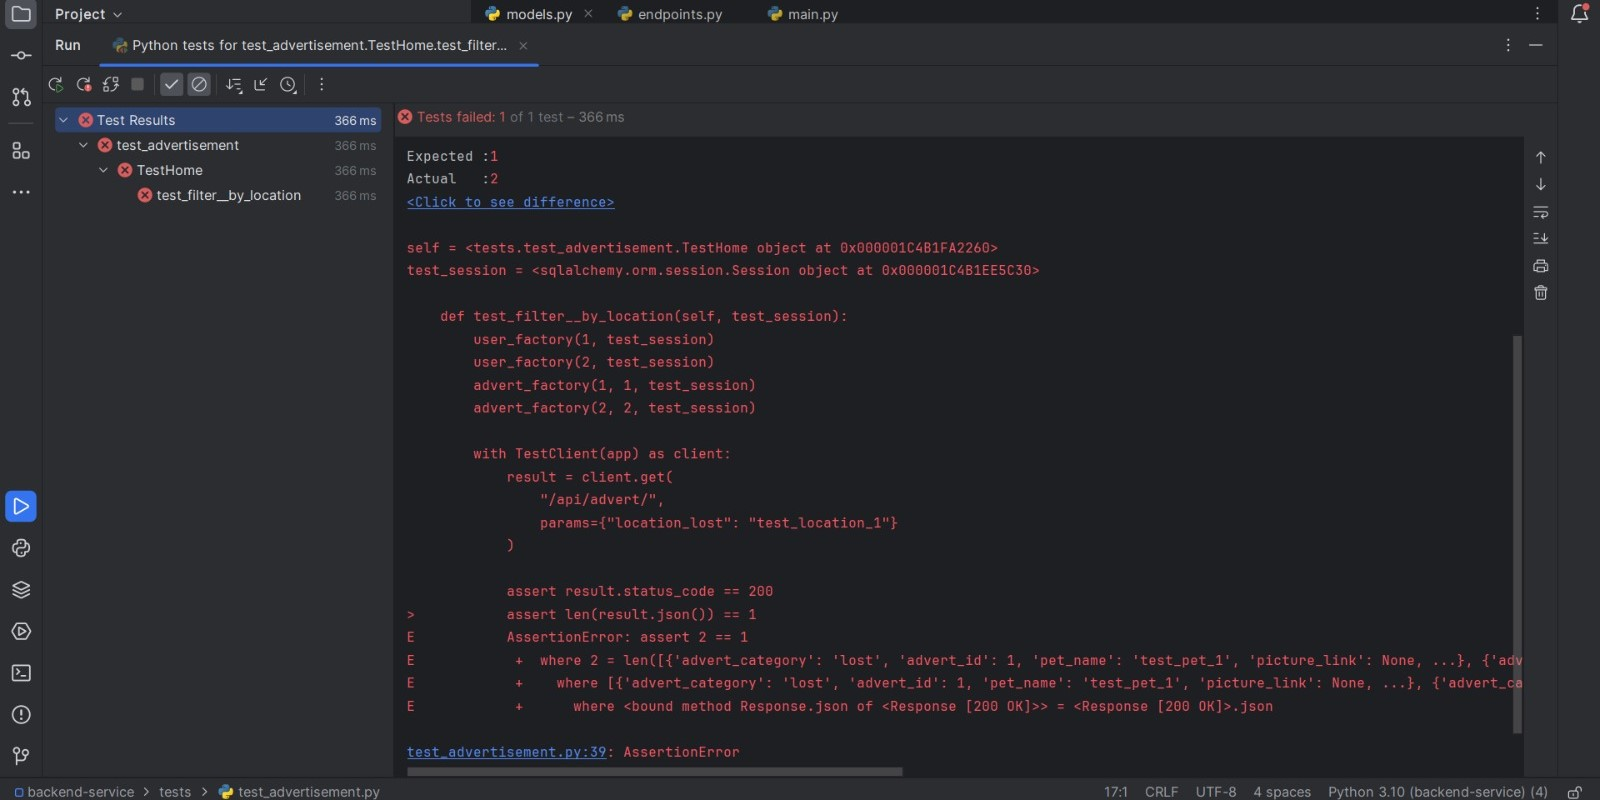
\includegraphics[scale=0.42]{slike/test8b.jpg} %veličina slike u odnosu na originalnu datoteku i pozicija slike
			 	\centering
			 	\caption{Rezultati testa 8. - 2. dio}
			 	\label{fig:test8b}
			 \end{figure}
			
			\subsection{Ispitivanje sustava}
			
			Ispitivanje sustava provedeno je ručno za sve obrasce uporabe. U nastavku su prikazani rezultati ispitivanja za UC2 (s UC15), UC3 (uključujući UC8), UC6 i UC9.

			\noindent \textbf{Ispitni  slučaj 1: Prijava korisnika u sustav}

			\noindent \textbf{Ulaz: }
			\begin{packed_enum}
				\item Otvaranje stranice za prijavu.
				\item Unos korisničkog imena i lozinke.
				\item Pritisak na gumb za prijavu.
			\end{packed_enum}

			\noindent \textbf{Očekivani rezultat: }
			\begin{packed_enum}
				\item Prikazuje se lista oglasa
				\item Odabirom ikone korisnika u \textit{toolbar-u} mogu se pregledati podaci o korisniku			
			\end{packed_enum}

			\noindent \textbf{Rezultat:} Očekivanja su zadovoljena. Aplikacija je prošla test.

			\begin{figure}[H]
			\centering
			\begin{minipage}{.5\textwidth}
	 			 \centering
				  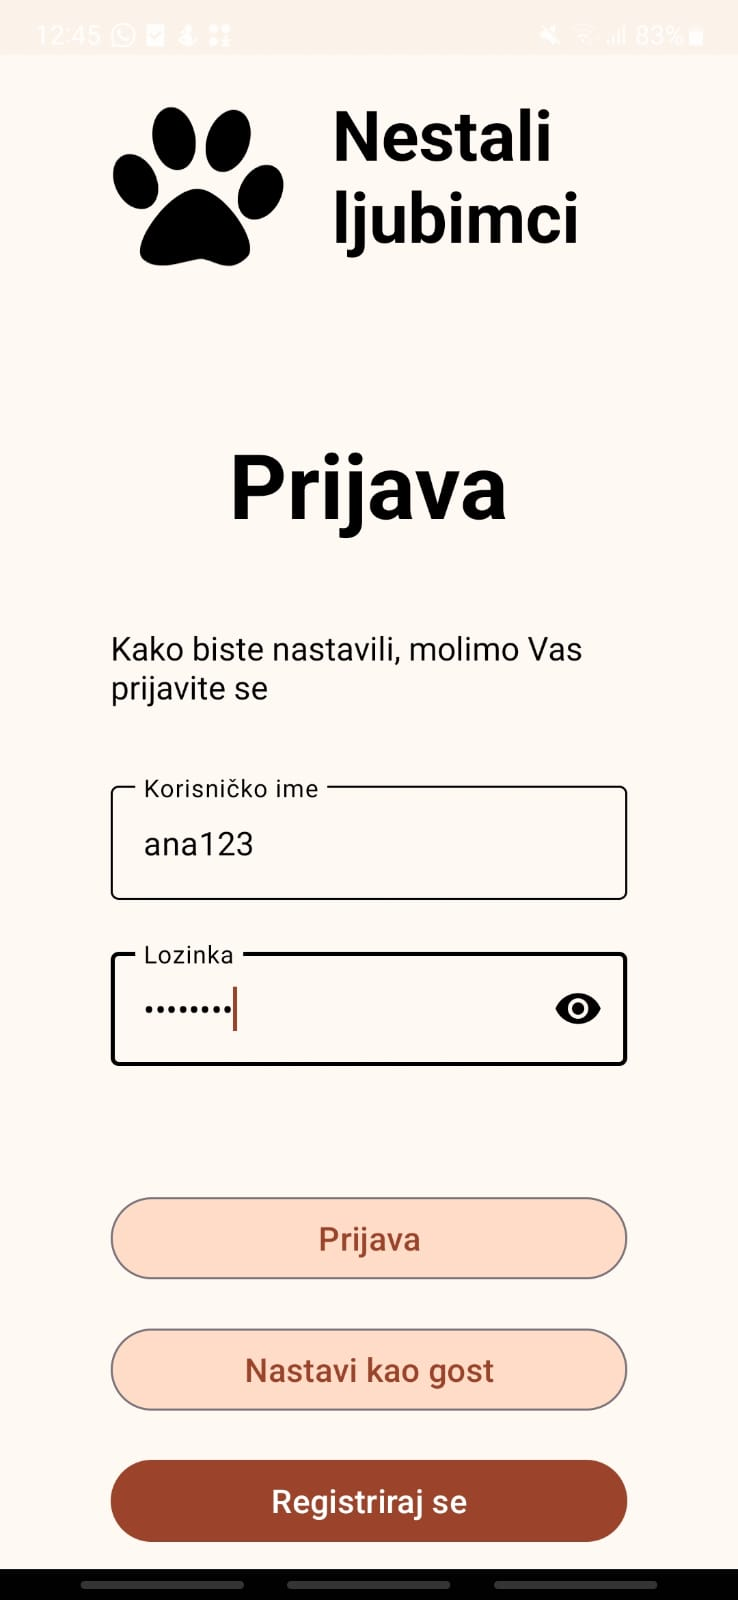
\includegraphics[width=.58\linewidth]{slike/app1v1.jpg}
				  \caption{Prijava u sustav}
				  \label{fig:app1v1}
			\end{minipage}%
			\begin{minipage}{.5\textwidth}
				  \centering
				  
\includegraphics[width=.58\linewidth]{slike/app1v2.jpg}
				  \caption{Prikaz profila}
				  \label{fig:app1v2}
			\end{minipage}
			\end{figure}

			\noindent \textbf{Ispitni  slučaj 2: Postavljanje oglasa}

			\noindent \textbf{Ulaz: }
			\begin{packed_enum}
				\item Odabir opcije "Dodaj oglas".
				\item Otvaranje forme za unos podataka.
				\item Unos podataka o nestalom ljubimcu.
				\item Pritisak na gumb za objavu oglasa.
			\end{packed_enum}

			\noindent \textbf{Očekivani rezultat: }
			\begin{packed_enum}
				\item[]\begin{packed_enum}
					\item	 Prikazuje se detaljni prikaz stvorenog oglasa.
					\item Nudi se mogućnost pisanja komentara.
				\end{packed_enum}	
			\end{packed_enum}

			\noindent \textbf{Rezultat:} Očekivanja su zadovoljena. Aplikacija je prošla test.

			\begin{figure}[H]
			\centering
			\begin{minipage}{.5\textwidth}
	 			 \centering
				  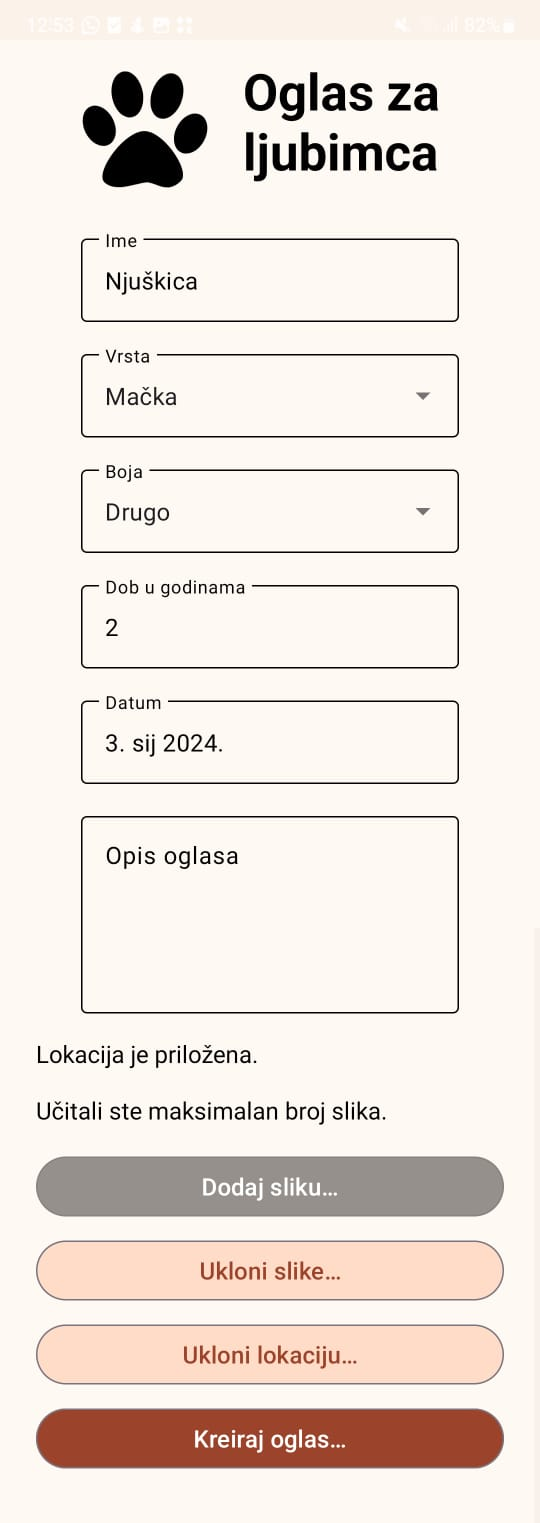
\includegraphics[width=.58\linewidth]{slike/app2v1.jpg}
				  \caption{Stvaranje novog oglasa}
				  \label{fig:app2v1}
			\end{minipage}%
			\begin{minipage}{.5\textwidth}
				  \centering
				  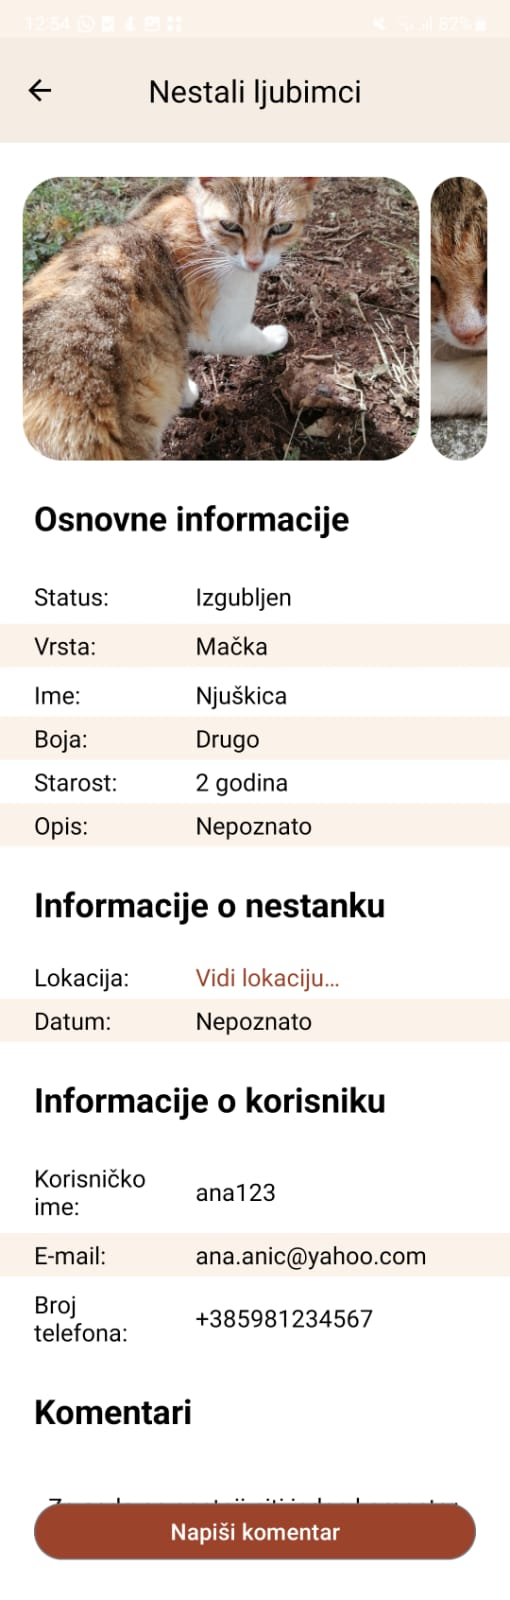
\includegraphics[width=.58\linewidth]{slike/app2v2.jpg}
				  \caption{Prikaz stvorenog oglasa}
				  \label{fig:app2v2}
			\end{minipage}
			\end{figure}

			\noindent \textbf{Ispitni  slučaj 3: Prikaz liste i pregled oglasa}

			\noindent \textbf{Ulaz: }
			\begin{packed_enum}
				\item Otvaranje aplikacije (već prijavljen korisnik ili odabir ulaska kao gost).
				\item Odabire se oglas za prikaz.
			\end{packed_enum}

			\noindent \textbf{Očekivani rezultat: }
			\begin{packed_enum}
				\item	 Prikazuje se lista svih oglasa.
				\item Prikazuje se detaljni prikaz odabranog oglasa.
			\end{packed_enum}

			\noindent \textbf{Rezultat:} Očekivanja su zadovoljena. Aplikacija je prošla test.

			\begin{figure}[H]
			\centering
			\begin{minipage}{.5\textwidth}
	 			 \centering
				  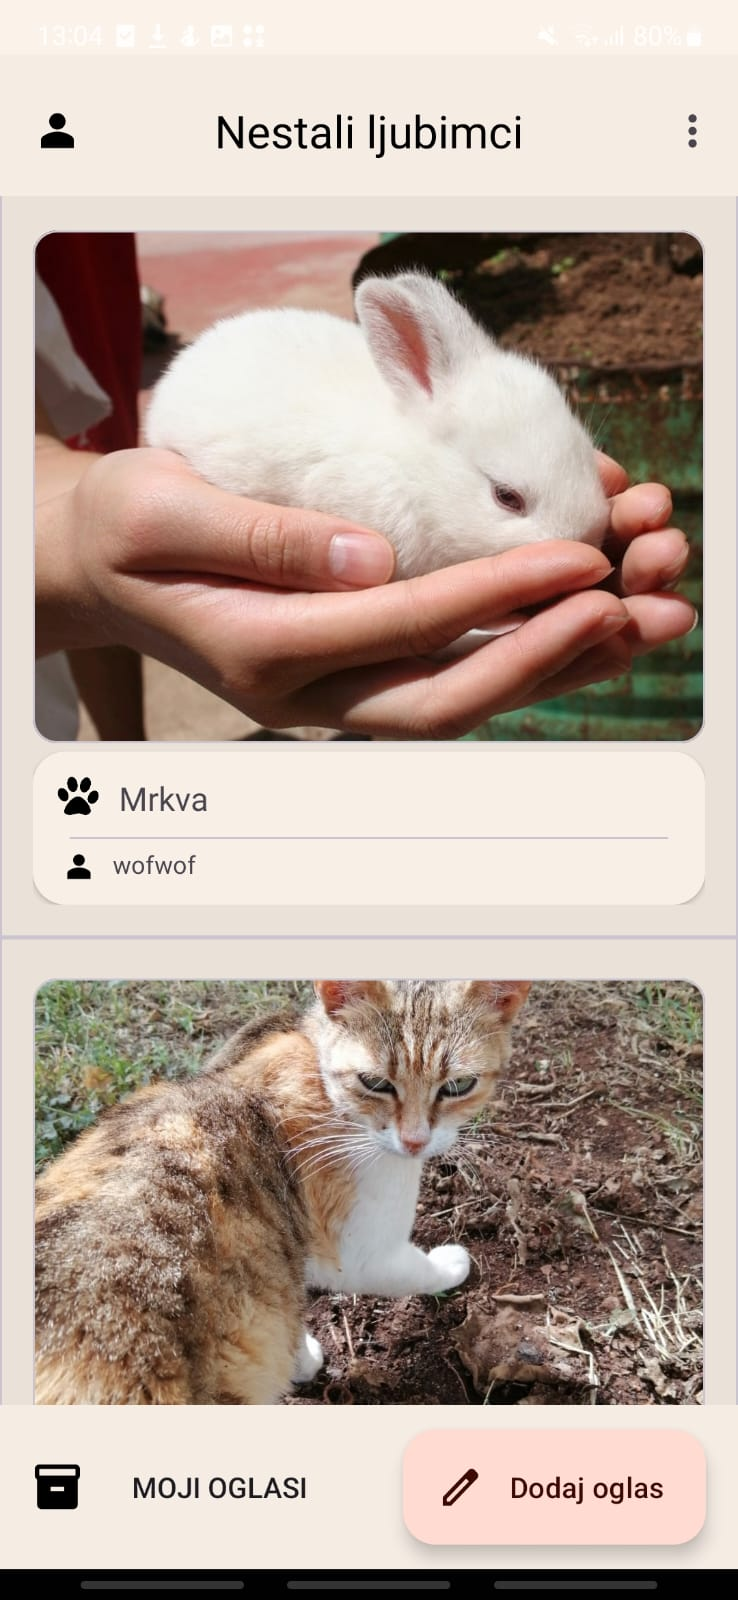
\includegraphics[width=.58\linewidth]{slike/app3v1.jpg}
				  \caption{Lista oglasa}
				  \label{fig:app3v1}
			\end{minipage}%
			\begin{minipage}{.5\textwidth}
				  \centering
				  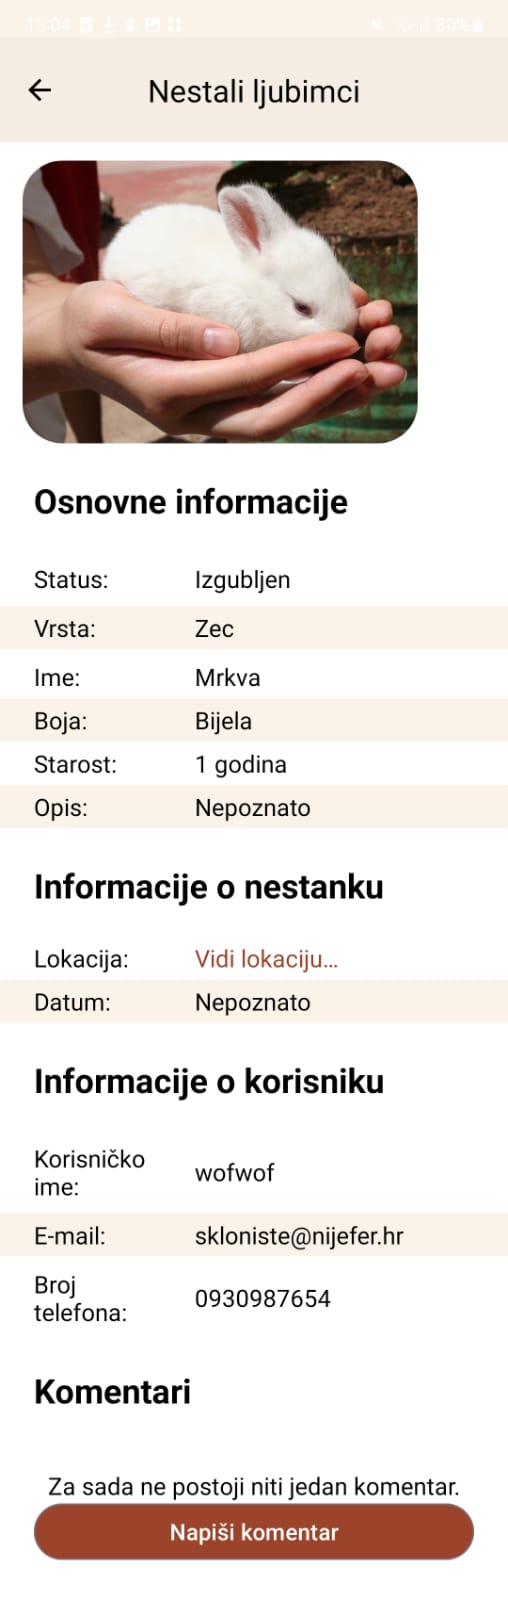
\includegraphics[width=.58\linewidth]{slike/app3v2.jpg}
				  \caption{Detaljni prikaz oglasa}
				  \label{fig:app3v2}
			\end{minipage}
			\end{figure}
			
			\noindent \textbf{Ispitni  slučaj 4: Brisanje oglasa}

			\noindent \textbf{Ulaz: }
			\begin{packed_enum}
				\item Pregled vlastitih oglasa.
				\item Odabir opcije za brisanje.
				\item Potvrda brisanja.
			\end{packed_enum}

			\noindent \textbf{Očekivani rezultat: }
			\begin{packed_enum}
				\item	[]\begin{packed_enum}
					\item	 Ispis poruke o uspješnom brisanju.
					\item Prikaz preostalih vlastitih oglasa ili poruka da ih više nema.
				\end{packed_enum}	
			\end{packed_enum}	

			\noindent \textbf{Rezultat:} Očekivanja su zadovoljena. Aplikacija je prošla test.

			\begin{figure}[H]
			\centering
			\begin{minipage}{.5\textwidth}
	 			 \centering
				  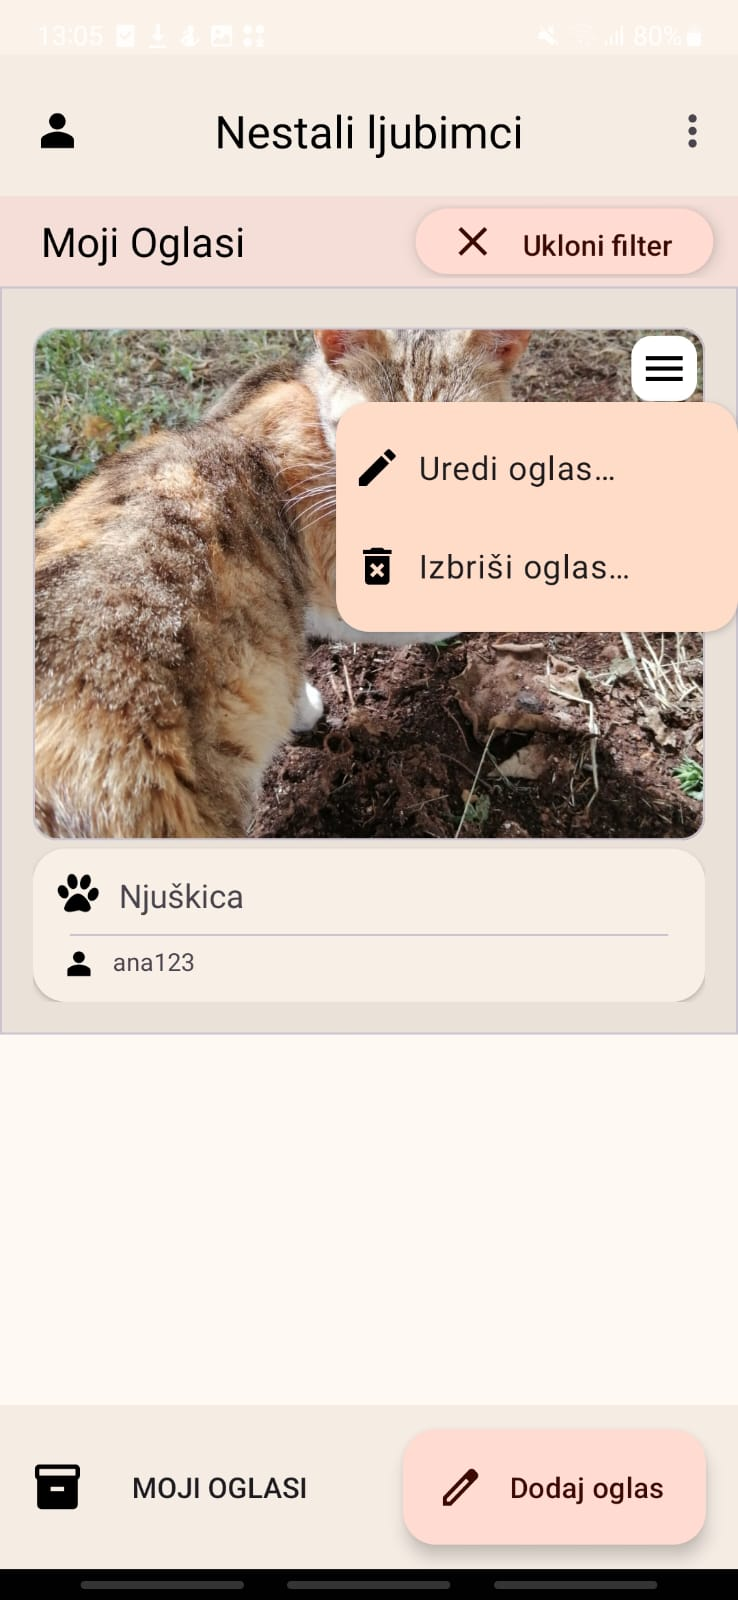
\includegraphics[width=.58\linewidth]{slike/app4v1.jpg}
				  \caption{Odabir brisanja}
				  \label{fig:app4v1}
			\end{minipage}%
			\begin{minipage}{.5\textwidth}
				  \centering
				  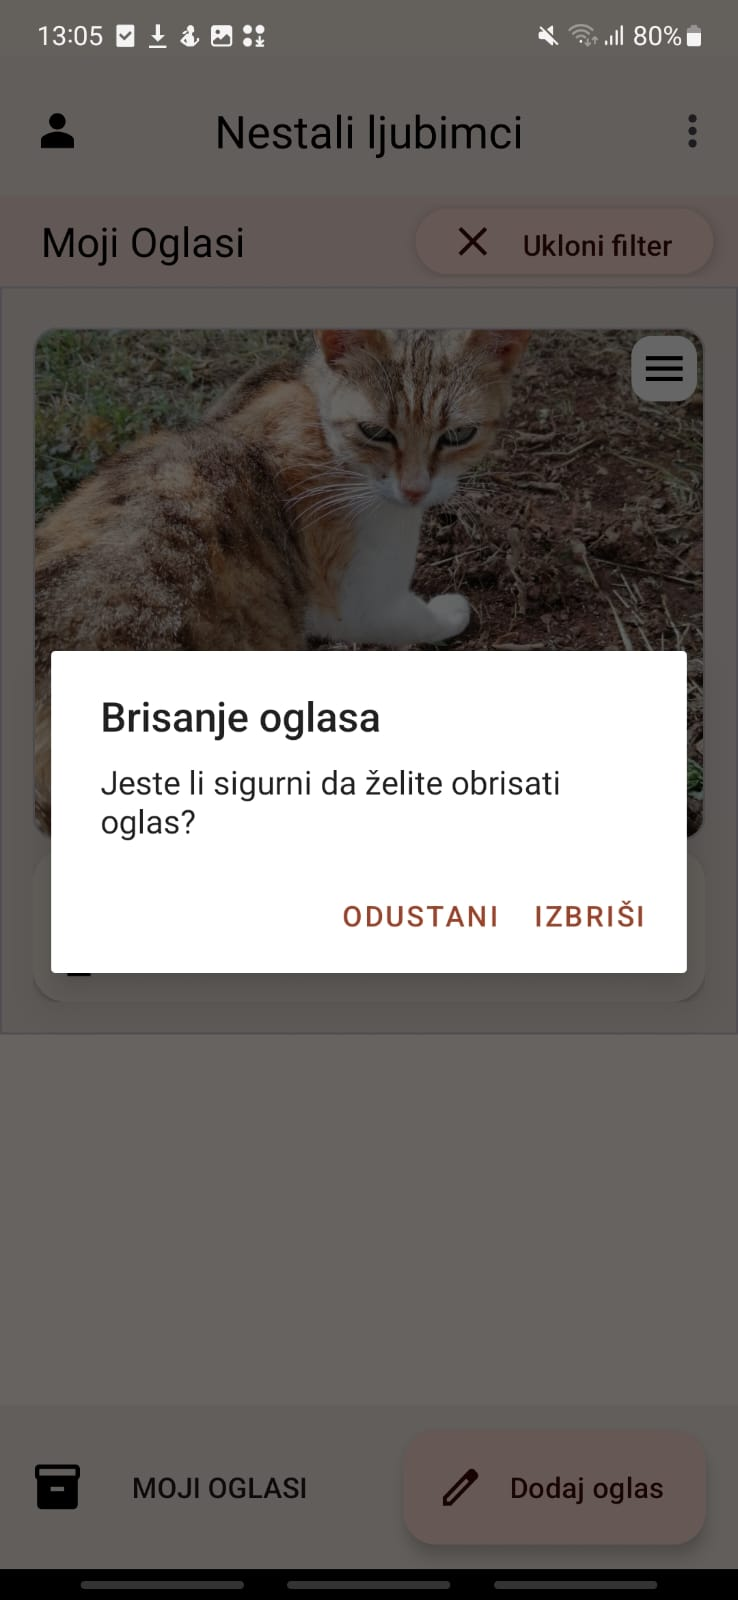
\includegraphics[width=.58\linewidth]{slike/app4v2.jpg}
				  \caption{Potvrda brisanja}
				  \label{fig:app4v2}
			\end{minipage}
			\end{figure}
			\begin{figure}[H]
				  
\includegraphics[scale=0.3]{slike/app4v3.jpg}
				  \centering
				  \caption{Prikaz preostalih oglasa}
				  \label{fig:app4v3}
			\end{figure}	 
			
			\eject 
		
		
		\section{Dijagram razmještaja}
			
			UML-dijagrami razmještaja prikazuju fizičku arhitekturu programskog sustava, prikazujući razmještaj programskih artefakata na sklopovskim čvorovima ili virtualnim okruženjima. Arhitektura sustava prepoznaje dvije različite funkcionalnosti - klijenta i poslužitelja. Korisnici pristupaju aplikaciji putem svojih mobilnih uređaja, dok se web poslužitelj i poslužitelj baze podataka nalaze na poslužiteljskom računalu. Komunikacija između korisnika aplikacije i poslužitelja odvija se putem HTTP veze.
			
			 \begin{figure}[H]
			 	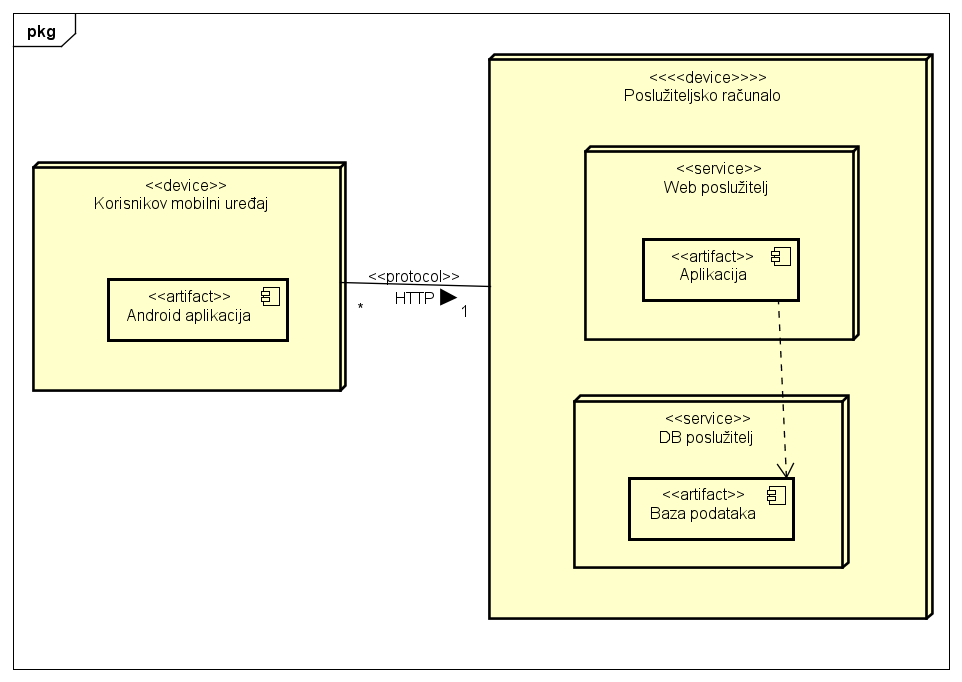
\includegraphics[scale=0.6]{dijagrami/dijagramRazmjestaja/dijagramRazmjestaja.PNG} %veličina slike u odnosu na originalnu datoteku i pozicija slike
			 	\centering
			 	\caption{Dijagram razmještaja}
			 	\label{fig:dRazmjestaja}
			 \end{figure}
			
			\eject 
		
		\section{Upute za puštanje u pogon}
		
		\subsection{Lokalni deploy aplikacije}
		
		\subsubsection{Baza podataka}
		
		Prije pokretanja backend servisa potrebno je lokalno stvoriti bazu podataka. Za to je potreban PostgreSQL poslužitelj baza podataka. Preporučamo dodatno korištenje grafičkih alata kao što su pgAdmin ili DBeaver, ali dovoljan je i samo PostgreSQL driver i konfiguracija iz komandne linije. Upute pratiti na službenim stranicama alata, ovisno o OS-u računala na kojem se pokreće.
		
		Nakon instalacije potrebno je stvoriti bazu podataka. Server očekuje da će se baza zvati „lost\_pets“, ali navedeno se može „pregaziti“ u settings.py fileu u root folderu backenda, u varijabli DEFAULT\_DATABASE. Ipak, preporučujemo da bazu nazovete „lost\_pets“.
		
		Ako se koristi pgAdmin, baza se može stvoriti odabirom „Servers“ $\rightarrow$ „PostgreSQL“ na lijevoj strani ekrana, a zatim desni klik na „PostgreSQL“ pa „Create“ $\rightarrow$ „Database“. Zatim se otvara prozor u kojem se unosi ime baze (\ref{fig:deploy1}) i nakon toga „Save“.
		
		\begin{figure}[H]
			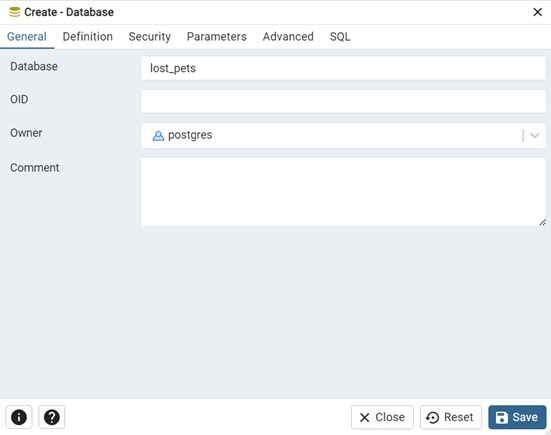
\includegraphics[scale=0.65]{slike/deploy1.jpg} %veličina slike u odnosu na originalnu datoteku i pozicija slike
			\centering
			\caption{Unos imena baze u pgAdminu}
			\label{fig:deploy1}
		\end{figure}
		
		User i password za pristup bazi su konfigurabilni, i preporučujemo mijenjati ih, ako je potrebno, u .env fileu, u varijablama POSTGRES\_USER i POSTGRES\_PASSWORD (Prilagoditi svojim PostgreSQL postavkama). Kako se postgres server defaultno nalazi na portu 5432, a bazu konfiguriramo lokalno, preporučujemo ostaviti POSTGRES\_HOST="localhost" te POSTGRES\_PORT=5432, iako se navedene postavke mogu i mijenjati.
		
		Ove se postavke kod deploya na remote poslužitelj također "pregaze" pomoću varijabli okruženja.
		
		Kada je sve od navedenog postavljeno, baza je spremna za početak rada servera. Tablice stvara repeatable skripta run\_migrations, a početne podatke ubacuje repeatable skripta init\_populate, koje se obje pokreću automatski kod pokretanja servisa.
		
		\subsubsection{Pokretanje servisa}
		
		Najlakši način za deploy servisa jest buildati Docker image iz Dockerfilea, a zatim pokrenuti Docker container iz spomenutog imagea. Ovo osigurava da će server imati sve što mu je potrebno i pokretati se u izoliranom okruženju. Upute za to pratiti na službenim Docker stranicama.
		
		Ovaj će se pristup skoro uvijek koristiti, i automatiziran je, kod deploya na remote server, a za detaljnije upute (poput postavljanja varijabli okruženja objašnjenih prije) potrebno je slijediti upute alata koji pruža usluge poslužitelja.
		
		Ipak, postoji relativno jednostavan način za pokretanje bez buildanja Docker image-a, a to je u virtualnom okruženju, uz lokalni python interpreter. Ukoliko ste na Linuxu, dovoljno će biti izvršiti sljedeće naredbe iz root foldera backenda (folder backend-service):
		
		\begin{lstlisting}
sudo apt-get update
sudo apt-get install python3
sudo apt-get install python3-pip
sudo apt install python3-venv
python3 -m venv ./venv
source venv/bin/activate
pip3 install -r requirements.txt
uvicorn service.main:app \end{lstlisting}

		Na windows OS-u pokretanje je nešto drugačije.
		
		Potrebno je imati instaliran python 3.10 (radi i sa 3.11) i odgovarajući pip installer.
		
		Nakon toga pozicionirati se u root folder backenda (backend-service) u command promptu i pokrenuti slijedno naredbe:
		
		\begin{lstlisting}
python -m venv ./venv
venv\Scripts\activate
pip install -r requirements.txt
uvicorn service.main:app \end{lstlisting}
		
		
		U oba slučaja servis bi se sada trebao nalaziti na http://localhost:8000, a Swagger dokumentacija (popis endpointa i mogućnost slanja direktnog requesta) dostupna je na http://localhost:8000/docs .
		
		\subsection{Postupak izgradnje i objave aplikacije}
		
		\subsubsection{Priprema za objavu}
		\begin{enumerate}
			\item[a)] Odabir ikone aplikacije
			\item[b)] Konfiguracija aplikacije
			
			Konfiguracija aplikacije uključuje: isključivanje debugginga
		\end{enumerate}
		
		\begin{figure}[H]
			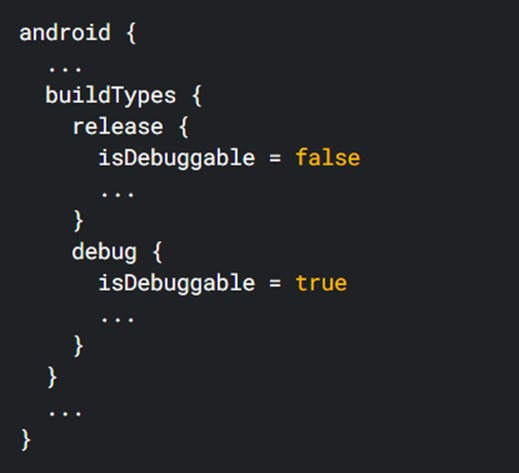
\includegraphics[scale=0.6]{slike/deploy2.jpg} %veličina slike u odnosu na originalnu datoteku i pozicija slike
			\centering
			\caption{Isključivanje logiranja, pregleda android manifesta te build opcija, odabir odgovarajučeg ID-a aplikacije.}
			\label{fig:deploy2}
		\end{figure}
		
		\subsubsection{Postavljanje verzije}
		
		\begin{figure}[H]
			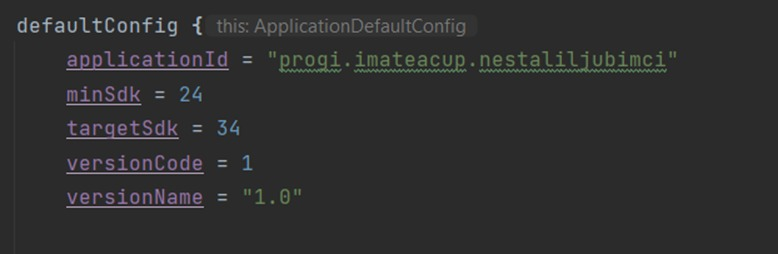
\includegraphics[scale=0.5]{slike/deploy3.jpg} %veličina slike u odnosu na originalnu datoteku i pozicija slike
			\centering
			\caption{Postavljanje verzije}
			\label{fig:deploy3}
		\end{figure}
		
		\subsubsection{Potpis aplikacije i release build aplikacije}
		
		Potrebno je generirati upload key i keystore, što je moguće korištenjem alata Android Studio.
		
		Nakon što je keystore generiran, moguće je izgraditi release verziju aplikacije u .aab ili .apk formatu. U Android Studiu odabrati \texttt{Build -> Select Build Variant} i odabrati "release". Zatim \texttt{Build -> Generate Signed Bundle(s) / Apk}, odabrati, u našem slučaju, APK.
		
		\begin{figure}[H]
			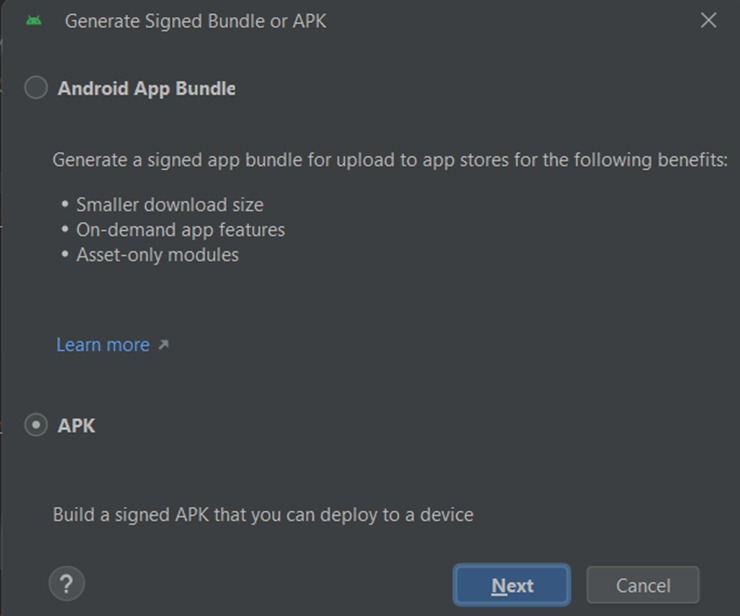
\includegraphics[scale=0.45]{slike/deploy4.jpg} %veličina slike u odnosu na originalnu datoteku i pozicija slike
			\centering
			\caption{Odabir APK}
			\label{fig:deploy4}
		\end{figure}
		
		Stisnuti \texttt{Next}, odabrati \texttt{key store path} koji vodi na ranije generirani keystore i unjeti \texttt{keystore}, \texttt{key password} i \texttt{alias}.
		
		\begin{figure}[H]
			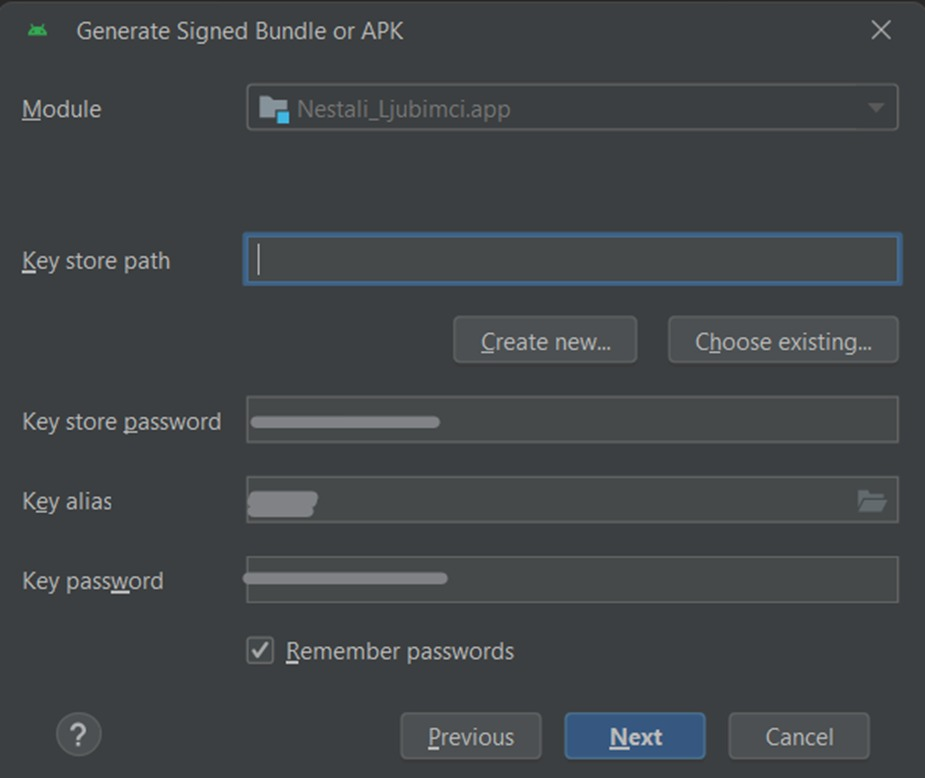
\includegraphics[scale=0.3]{slike/deploy5.jpg} %veličina slike u odnosu na originalnu datoteku i pozicija slike
			\centering
			\caption{Unos za keystore, key password i allias}
			\label{fig:deploy5}
		\end{figure}
		
		Stisnuti \texttt{Next}, odabrati \texttt{build variant}, odredišni folder i kliknuti \texttt{Create}. Potpisani APK će se nalaziti u specificiranom folderu.
		
		\begin{figure}[H]
			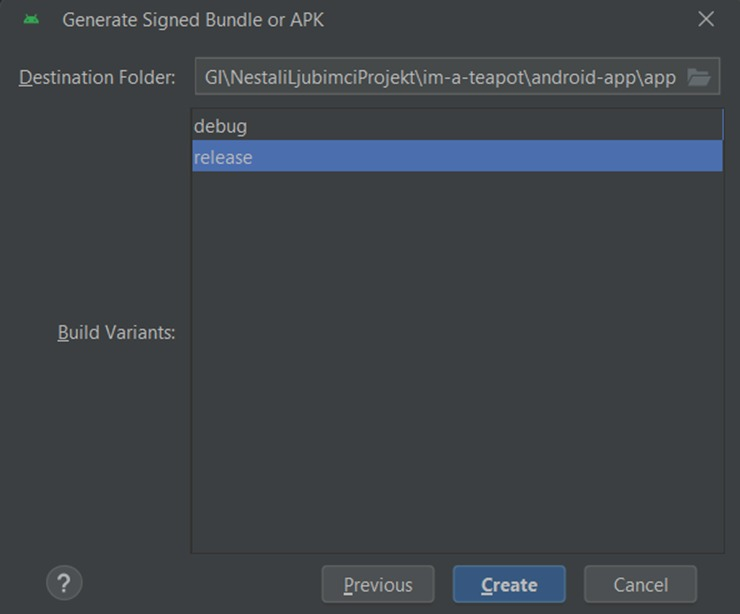
\includegraphics[scale=0.43]{slike/deploy6.jpg} %veličina slike u odnosu na originalnu datoteku i pozicija slike
			\centering
			\caption{Odabir mape za APK i izrada}
			\label{fig:deploy6}
		\end{figure}
		
		\subsubsection{Objava aplikacije na odabranom appstore-u}
		
		Objava aplikacije znatno se razlikuje na različitim trgovinama aplikacija, a postupak objave često je rigorozan te se nerijetko plaća. Zbog takve kompleksnosti i spomenutih razlika u procesu objave, nećemo ulaziti u detalje već ćemo ukratko opisati postupak objave na Amazon Appstoreu.
		
		Za početak, potrebno je napraviti račun na Amazon Appstoreu te se navigirati na sljedeću stranicu: \sloppy\url{https://developer.amazon.com/docs/app-submission/submitting-apps-to-amazon-appstore.html}.
		
		Prateći upute na priloženoj stranici, potrebno se ulogirati u Amazon Developer konzolu. Zatim kliknuti na \textit{dashboard} te nakon toga odabrati \textit{Add a New App} iz padajućeg izbornika i odabrati \textit{Android}. Ponovno odabrati \textit{Add a New App} te \textit{Android}. Zatim je potrebno pratiti formu te ispuniti sva polja koja Amazon zahtijeva te generirati zahtjev za objavu. Nakon što se to uspješno obavi, potrebno je čekati da Amazon Appstore odobri upload aplikacije.
		
		
		\eject
		
	\chapter{Zaključak i budući rad}
		
		\textbf{\textit{dio 2. revizije}}\\
		
		...
		
		\eject 
	\chapter*{Popis literature}
		\addcontentsline{toc}{chapter}{Popis literature}
	 	
		
		
		\begin{enumerate}
			
			
			\item  Programsko inženjerstvo, FER ZEMRIS, \url{http://www.fer.hr/predmet/proinz}
			
			\item  MissingPetApp, \url{https://missingpet.app/}

			\item  GeeksforGeeks, MVC (Model View Controller) Architecture Pattern in Android, \url{https://www.geeksforgeeks.org/mvc-model-view-controller-architecture-pattern-in-android-with-example/?ref=lbp}
			
		\end{enumerate}
		
		 
	
	
	\begingroup
	\renewcommand*\listfigurename{Indeks slika i dijagrama}
	%\renewcommand*\listtablename{Indeks tablica}
	%\let\clearpage\relax
	\listoffigures
	%\vspace{10mm}
	%\listoftables
	\endgroup
	\addcontentsline{toc}{chapter}{Indeks slika i dijagrama}


	
	\eject 
		
	\chapter*{Dodatak: Prikaz aktivnosti grupe}
		\addcontentsline{toc}{chapter}{Dodatak: Prikaz aktivnosti grupe}
		
		\section*{Dnevnik sastajanja}
		
		
		\begin{packed_enum}
			\item  sastanak
			
			\item[] \begin{packed_item}
				\item Datum: 16. listopada 2023.
				\item Prisustvovali: N. Ivić, M. Krajinović, M. Matulić, B. Mikan, A. Radoš, M. Žagar, I. Žinić
				\item Teme sastanka:
				\begin{packed_item}
					\item  sastanak s asistentom i demonstratorom
					\item  raspodijela zadataka 
					\item  dogovor o korištenim tehnologijama
				\end{packed_item}
			\end{packed_item}
			
			\item  sastanak
			\item[] \begin{packed_item}
				\item Datum: 19. listopada 2023.
				\item Prisustvovali: B. Mikan, A. Radoš, M. Žagar
				\item Teme sastanka:
				\begin{packed_item}
					\item  uvod u frontend tehnologije
					\item  uvod u proces razvoja frontenda
				\end{packed_item}
			\end{packed_item}
			
			\item  sastanak
			\item[] \begin{packed_item}
				\item Datum: 21. listopada 2023.
				\item Prisustvovali: N. Ivić, M. Krajinović
				\item Teme sastanka:
				\begin{packed_item}
					\item  dogovorena struktura backend dijela aplikacije
					\item  objašnjen fastapi i sqlalchemy
					\item  detaljnije dogovorena podjela posla u podtimu
				\end{packed_item}
			\end{packed_item}

			\item  sastanak
			\item[] \begin{packed_item}
				\item Datum: 23. listopada 2023.
				\item Prisustvovali: N. Ivić, M. Krajinović, M. Matulić, B. Mikan, A. Radoš, M. Žagar, I. Žinić
				\item Teme sastanka:
				\begin{packed_item}
					\item  dogovaranje detalja oko implementacije
					\item  raščišćavanje osnovnih dilema funkcionalnosti 
				\end{packed_item}
			\end{packed_item}

			\item  sastanak
			\item[] \begin{packed_item}
				\item Datum: 25. listopada 2023.
				\item Prisustvovali: M. Matulić, I. Žinić
				\item Teme sastanka:
				\begin{packed_item}
					\item  detaljnija razrada opisa zadatka
					\item  raspisivanje funkcionalnih zahtjeva i opis obrazaca uporabe
				\end{packed_item}
			\end{packed_item}
			
			\item  sastanak
			\item[] \begin{packed_item}
				\item Datum: 28. listopada 2023.
				\item Prisustvovali: B. Mikan, A. Radoš, M. Žagar
				\item Teme sastanka:
				\begin{packed_item}
					\item  diskusija oko dizajniranja sučelja u alatu figma
					\item  uvod u proces razvoja frontenda
					\item  odabir color palete
					\item  generalni apstraktni plan arhitekture aplikacije
					\item  branch naming konvencija
					\item  podijeljeni prvi jira taskovi
				\end{packed_item}
			\end{packed_item}
			
			\item  sastanak
			\item[] \begin{packed_item}
				\item Datum: 6. studenoga 2023.
				\item Prisustvovali: N. Ivić, M. Krajinović, M. Matulić, B. Mikan, A. Radoš, M. Žagar, I. Žinić
				\item Teme sastanka:
				\begin{packed_item}
					\item  rješavanje nesuglasica
					\item  daljnja raspodjela posla
					\item  dogovor oko budućih uvjeta zadatka
					\item  uvod u tehnički proces puštanja aplikacije u pogon
				\end{packed_item}
			\end{packed_item}
			
			\item  sastanak
			\item[] \begin{packed_item}
				\item Datum: 13. studenoga 2023.
				\item Prisustvovali: N. Ivić, M. Krajinović, M. Matulić, B. Mikan, A. Radoš, M. Žagar, I. Žinić
				\item Teme sastanka:
				\begin{packed_item}
					\item  organizacija puštanja aplikacije u pogon
					\item  testiranje aplikacije
					\item  provjera detalja aplikacije i dokumentacije
				\end{packed_item}
			\end{packed_item}
			
			\item  sastanak
			\item[] \begin{packed_item}
				\item Datum: 4. prosinca 2023.
				\item Prisustvovali: N. Ivić, M. Krajinović, M. Matulić, B. Mikan, A. Radoš, I. Žinić
				\item Teme sastanka:
				\begin{packed_item}
					\item  daljnja raspodjela posla
					\item  dogovori između frontenda i backenda
				\end{packed_item}
			\end{packed_item}
			
			\item  sastanak
			\item[] \begin{packed_item}
				\item Datum: 11. prosinca 2023.
				\item Prisustvovali: N. Ivić, M. Krajinović, M. Matulić, B. Mikan, A. Radoš, M. Žagar
				\item Teme sastanka:
				\begin{packed_item}
					\item  pregled grešaka prve revizije
					\item  razgovor s profesorom
					\item  planiranje budućeg rada
				\end{packed_item}
			\end{packed_item}

			\item  sastanak
			\item[] \begin{packed_item}
				\item Datum: 18. prosinca 2023.
				\item Prisustvovali: N. Ivić, M. Krajinović, M. Matulić, B. Mikan, A. Radoš, M. Žagar, I. Žinić
				\item Teme sastanka:
				\begin{packed_item}
					\item  pregled do sada obavljenog dijela
					\item  daljnja raspodjela posla
					\item  planiranje budućeg rada
				\end{packed_item}
			\end{packed_item}
			
			\item  sastanak
			\item[] \begin{packed_item}
				\item Datum: 8. siječnja 2024.
				\item Prisustvovali: N. Ivić, M. Krajinović, M. Matulić, B. Mikan, M. Žagar
				\item Teme sastanka:
				\begin{packed_item}
					\item  pregled do sada obavljenog posla
					\item  dogovor oko testiranja i deploymenta
					\item  rješavanje pitanja u vezi dokumentacije
				\end{packed_item}
			\end{packed_item}
			
			\item  sastanak
			\item[] \begin{packed_item}
				\item Datum: 15. siječnja 2024.
				\item Prisustvovali: N. Ivić, M. Krajinović, M. Matulić, B. Mikan, A. Radoš, M. Žagar, I. Žinić
				\item Teme sastanka:
				\begin{packed_item}
					\item  pregled do sada obavljenog posla
					\item  rješavanje nesuglasica
					\item  planiranje zadnjeg tjedna rada
					\item  dogovori oko prezentacije
				\end{packed_item}
			\end{packed_item}
			
			%
			
		\end{packed_enum}
		
		\eject
		\section*{Tablica aktivnosti}
		
			
			 \textit{Napomena: Doprinosi u tablici su navedeni u satima.}

			\begin{longtblr}[
					label=none,
				]{
					vlines,hlines,
					width = \textwidth,
					colspec={X[7, l]X[1, c]X[1, c]X[1, c]X[1, c]X[1, c]X[1, c]X[1, c]}, 
					vline{1} = {1}{text=\clap{}},
					hline{1} = {1}{text=\clap{}},
					rowhead = 1,
				} 
			
				\SetCell[c=1]{c}{} & \SetCell[c=1]{c}{\rotatebox{90}{\textbf{Nora Ivić}}} & \SetCell[c=1]{c}{\rotatebox{90}{\textbf{Mirta Krajinović }}} &	\SetCell[c=1]{c}{\rotatebox{90}{\textbf{Marta Matulić }}} & \SetCell[c=1]{c}{\rotatebox{90}{\textbf{Bruno Mikan }}} &	\SetCell[c=1]{c}{\rotatebox{90}{\textbf{Antonio Radoš }}} & \SetCell[c=1]{c}{\rotatebox{90}{\textbf{Marko Žagar }}} &	\SetCell[c=1]{c}{\rotatebox{90}{\textbf{Ivan Žinić }}} \\  
				Upravljanje projektom 		& 9 &  &  &  &  &  & \\ 
				Opis projektnog zadatka 	&  &  & 7 &  &  &  & 3 \\ 
				
				Funkcionalni zahtjevi       &  &  & 2 &  &  &  & 6 \\ 
				Opis pojedinih obrazaca 	&  &  & 2 &  &  &  & 6 \\ 
				Dijagram obrazaca 			&  &  &  &  &  &  & 8 \\ 
				Sekvencijski dijagrami 		&  &  & 6 &  &  &  & 1 \\ 
				Opis ostalih zahtjeva 		&  &  & 2 &  &  &  &  \\ 

				Arhitektura i dizajn sustava	 &  &  & 6 &  &  &  & 1 \\ 
				Opći prioriteti i svrha sustava  & 2 & 2 & 5 & 2 & 2 & 2 & 5 \\ 
				Dizajn baze podataka			& 2 & 10 & 2 &  &  &  &   \\ 
				Dokumentacija baze podataka	&  & 2 & 7 &  &  &  & 7  \\ 
				Dijagram razreda 			& 1 &  & 8 & 2 &  &  & 8  \\ 
				Dijagram stanja				&  &  &  &  &  &  &  \\ 
				Dijagram aktivnosti 		&  &  &  &  &  &  &  \\ 
				Dijagram komponenti			&  &  &  &  &  &  &  \\ 
				Korištene tehnologije i alati 		& 8 & 7 & 6 & 7 & 9 & 9 & 6 \\ 
				Ispitivanje programskog rješenja 	& 7 & 7 & 2 & 5 & 5 & 5 & 2 \\ 
				Dijagram razmještaja			&  &  &  &  &  &  &  \\ 
				Upute za puštanje u pogon 		& 1 &  &  &  &  &  &  \\  
				Plan rada					 & 10 & 10 & 10 & 15 & 15 & 15 & 10 \\ 
				Dnevnik sastajanja 			&  &  & 1 &  &  &  & 3 \\ 
				Zaključak i budući rad 		&  &  &  &  &  &  &  \\  
				Popis literature 			&  &  & 1 &  &  &  &  \\  

				Definiranje endpointa		& 4 &  &  &  &  &  &  \\ 
				Izrada baze podataka			&  & 15 &  &  &  &  &  \\ 
				Spajanje s bazom 				& 3 & 3 &  &  &  &  &  \\  
				Backend		 			& 10 &  &  &  &  &  & \\  
				Deployment			& 6 & 6 &  &  &  &  &  \\ 
				Dizajn izgleda aplikacije			&  &  &  & 7 & 8 & 5 &  \\  
				Implementacija izgleda			&  &  &  & 20 & 18 & 17 &\\ 
				Povezivanje s backendom			&  &  &  & 6 & 6 & 6 &\\ 
			\end{longtblr}
					
					
		\eject
		\section*{Dijagrami pregleda promjena}
		
		\textbf{\textit{dio 2. revizije}}\\
		
		Github dijagrami...
		
	


\end{document} %naredbe i tekst nakon ove naredbe ne ulaze u izgrađen dokument 


